%! Author = dboldog, tbubenik
%! Date = 16/02/2026

\documentclass[11pt, a4paper]{article}

% ─── Packages ────────────────────────────────────────────────────────────────
\usepackage[utf8]{inputenc}
\usepackage[T1]{fontenc}
\usepackage[margin=2.5cm]{geometry}
\usepackage{graphicx}
\usepackage{hyperref}
\usepackage{booktabs}       % nicer tables (\toprule, \midrule, \bottomrule)
\usepackage{float}          % [H] placement for figures and tables
\usepackage{xcolor}         % colors (used by listings)
\usepackage{listings}       % code listings
\hypersetup{colorlinks=true, linkcolor=black, citecolor=black, urlcolor=blue!70!black}

% ─── Code listing style ─────────────────────────────────────────────────────
\lstset{
    basicstyle=\ttfamily\small,
    breaklines=true,
    frame=single,
    numbers=left,
    numberstyle=\tiny\color{gray},
    xleftmargin=2em,
    framexleftmargin=1.5em
}
% Pro tip: for syntax highlighting, look into the 'minted' package.

% ─── Bibliography ────────────────────────────────────────────────────────────
\usepackage[style=numeric, backend=bibtex]{biblatex}
\addbibresource{references.bib}
 
% ─── Language (swap to lang/sk for Slovak) ───────────────────────────────────
% Slovak language pack
\usepackage[slovak]{babel}

\newcommand{\LabelProtocol}{Protokol k zadaniu}
\newcommand{\LabelCourse}{Databázové technológie}
\newcommand{\LabelCode}{DBS}
\newcommand{\LabelUniversity}{Slovenská technická univerzita v~Bratislave}
\newcommand{\LabelFaculty}{Fakulta informatiky a~informačných technológií}
\newcommand{\LabelAssignment}{Zadanie}
\newcommand{\LabelStudent}{Študent}
\newcommand{\LabelTeacher}{Cvičiaci}
\newcommand{\LabelGroup}{Študijná skupina}
\newcommand{\LabelDate}{Dátum}
\newcommand{\LabelYear}{Akademický rok}
\newcommand{\LabelContents}{Obsah}

% ─── Student details ─────────────────────────────────────────────────────────
\newcommand{\StudentName}{Dávid Boldog, Tomáš Bubeník}
\newcommand{\StudyGroup}{Štvrtok 11:00}
\newcommand{\TeacherName}{Ing. Matej Petrík}
\newcommand{\AssignmentNumber}{1}
\newcommand{\AssignmentTitle}{Reštauračný systém}
\newcommand{\AcademicYear}{2025/2026}

% =============================================================================
\begin{document}

% ─── Cover page ──────────────────────────────────────────────────────────────
\begin{titlepage}
    \centering

    \includegraphics[width=0.3\textwidth]{../assets/logo}

    \vspace{0.3cm}
    {\large \LabelUniversity}\\[2pt]
    {\large \LabelFaculty}

    \vspace{2.5cm}
    {\Huge\bfseries \LabelProtocol}

    \vspace{0.6cm}
    {\LARGE \LabelCode{} --- \LabelCourse}

    \vspace{0.4cm}
    {\Large \LabelAssignment{} \AssignmentNumber: \AssignmentTitle}

    \vfill

    \begin{tabular}{r l}
        \textbf{\LabelStudent:} & \StudentName  \\[4pt]
        \textbf{\LabelGroup:}   & \StudyGroup   \\[4pt]
        \textbf{\LabelTeacher:} & \TeacherName  \\[4pt]
        \textbf{\LabelYear:}    & \AcademicYear \\[4pt]
        \textbf{\LabelDate:}    & \today        \\
    \end{tabular}

    \vspace{1.5cm}
\end{titlepage}

% ─── Table of contents ───────────────────────────────────────────────────────
\renewcommand{\contentsname}{\LabelContents}
\tableofcontents
\newpage

% =============================================================================

\section{Špecifikácia}
\label{sec:specifikacia}

Reštauračný systém rieši problém evidencie a riadenia prevádzkových procesov 
v reštauračnom zariadení. Systém je určený pre reštaurácie, ktoré chcú 
digitalizovať svoju prevádzku — od správy stolov a rezervácií až po spracovanie 
objednávok a platieb. Jeho pridaná hodnota spočíva v tom, že zjednocuje všetky 
prevádzkové procesy do jedného nástroja, znižuje chybovosť spôsobenú ručným 
zadávaním, zrýchľuje obsluhu zákazníkov a poskytuje manažmentu prehľad 
o prevádzke v reálnom čase. Systém podporuje dva prevádzkové modely --- 
klasickú obsluhu pri stole (\textbf{dine-in}) a donáškový servis 
(\textbf{delivery}).

% ─────────────────────────────────────────────────────────────────────────────
\subsection{Aktéri systému}

Systém rozlišuje päť typov aktérov, pričom každý má presne vymedzenú rolu, 
zodpovednosti a úroveň prístupu.

\begin{itemize}

    \item \textbf{Zákazník} je koncový používateľ systému, ktorý vytvára 
    rezervácie stolov, prezerá jedálniček, zadáva objednávky a realizuje 
    platby. Má prístup výlučne k vlastným objednávkam, rezerváciám 
    a platobným záznamom. V prípade donášky môže sledovať stav svojej 
    objednávky a po jej doručení zanechať recenziu.

    \item \textbf{Čašník} je zamestnanec zodpovedný za priamu obsluhu 
    zákazníkov pri stoloch. Spravuje priradenie zákazníkov k stolom, zadáva 
    a modifikuje objednávky v mene zákazníka a iniciuje platobný proces. 
    Má prístup k zoznamu stolov a ich stavom a k aktívnym objednávkam.

    \item \textbf{Kuchár} prijíma objednávky zaradené do frontu a zodpovedá 
    za ich prípravu. Jeho úlohou v systéme je zmeniť stav objednávky 
    z \textit{„čaká na prípravu"} na \textit{„pripravuje sa"} a po dokončení 
    na \textit{„hotová"}. Kuchár má prístup iba k identifikátoru objednávky 
    a zoznamu objednaných položiek --- osobné údaje zákazníka sú pre neho 
    skryté.

    \item \textbf{Manažér} má najvyššiu úroveň prístupu v systéme. 
    Zodpovedá za správu jedálničku, kontrolu skladových zásob, správu 
    zamestnancov a generovanie prevádzkových reportov. Môže pristupovať 
    ku všetkým dátam v systéme.

    \item \textbf{Kuriér} zabezpečuje fyzické doručenie objednávok na adresu 
    zákazníka. Systém mu sprístupní iba informácie nevyhnutné pre doručenie 
    --- doručovaciu adresu, spôsob platby a kontaktné údaje zákazníka. 
    Po odovzdaní objednávky aktualizuje jej stav na \textit{„doručená"}.

\end{itemize}

% ─────────────────────────────────────────────────────────────────────────────
\subsection{Kľúčové entity}

Systém eviduje niekoľko kľúčových entít, ktoré spoločne pokrývajú celý 
životný cyklus reštauračnej prevádzky.

\begin{itemize}

    \item \textbf{Zákazník} reprezentuje identitu osoby interagujúcej 
    so systémom. Evidujeme jeho osobné a kontaktné údaje vrátane doručovacej 
    adresy, ktorá je nevyhnutná pre objednávky typu delivery.

    \item \textbf{Zamestnanec} zastupuje všetkých pracovníkov reštaurácie. 
    Rola je evidovaná ako atribút zamestnanca, čo zjednodušuje správu 
    prístupových práv a personálnych záznamov.

    \item \textbf{Stôl} reprezentuje fyzickú kapacitu reštaurácie. 
    Evidujeme číslo stola, jeho kapacitu a aktuálny stav --- 
    \textit{voľný}, \textit{rezervovaný} alebo \textit{obsadený}.

    \item \textbf{Rezervácia} zachytáva plánované využitie konkrétneho stola 
    v stanovenom časovom intervale. Je prepojená so zákazníkom a stolom 
    a obsahuje dátum, čas začiatku a konca. Táto entita je kritická pre 
    správne riadenie kapacity reštaurácie.

    \item \textbf{Objednávka} je ústrednou entitou celého systému. Môže byť 
    typu \textbf{dine-in} (prepojená so stolom a čašníkom) alebo 
    \textbf{delivery} (prepojená s adresou a kuriérom). Eviduje stav 
    spracovania a časové pečiatky jednotlivých prechodov.

    \item \textbf{Položka menu} predstavuje ponuku reštaurácie --- každé 
    jedlo alebo nápoj s názvom, popisom, cenou a kategóriou. Systém uchováva históriu zmien cien\footnote{Cena položky je pri vytvorení objednávky uložená ako snímka hodnoty v čase objednávky, aby historické objednávky zostali konzistentné aj po zmene ceny v menu.}, aby staré objednávky zostali konzistentné.

    \item \textbf{Platba} zaznamenáva úhradu spojenú s konkrétnou 
    objednávkou. Eviduje celkovú sumu, spôsob platby, časovú pečiatku 
    a stav platby.

    \item \textbf{Recenzia} umožňuje zákazníkovi ohodnotiť skúsenosť po 
    dokončení objednávky. Je prepojená s konkrétnou objednávkou\footnote{Prepojenie zabezpečuje, že recenziu môže zanechať iba zákazník, ktorý skutočne uskutočnil objednávku.}, čím sa 
    zabraňuje viacnásobnému hodnoteniu tej istej návštevy.

\end{itemize}

% ─────────────────────────────────────────────────────────────────────────────
\subsection{Biznis pravidlá a obmedzenia}

Systém musí rešpektovať niekoľko biznis pravidiel, ktoré sa priamo premietajú 
do integritných obmedzení databázy.

\begin{itemize}

    \item \textbf{Exkluzivita rezervácií} --- stôl nemôže byť rezervovaný 
    pre viac ako jednu rezerváciu v rovnakom časovom intervale. Obmedzenie 
    sa implementuje ako kontrola prekrývania časových intervalov pre daný stôl.

    \item \textbf{Podmienka vytvorenia objednávky} --- objednávku typu 
    dine-in je možné vytvoriť iba pre stôl v stave \textit{„rezervovaný"} 
    alebo \textit{„obsadený"}. Zabraňuje sa tým vzniku objednávok pre 
    stoly, pri ktorých nesedí žiadny zákazník.

    \item \textbf{Podmienka uzavretia objednávky} --- objednávka nemôže 
    byť označená ako \textit{„zaplatená"}, pokiaľ k nej neexistuje platný 
    záznam o platbe. Obmedzenie sa vynucuje cudzím kľúčom a stavovým 
    automatom objednávky.

    \item \textbf{Dostupnosť skladových zásob} --- položku menu nie je 
    možné zaradiť do objednávky, ak nie sú dostupné potrebné ingrediencie 
    na sklade. Po potvrdení objednávky systém zodpovedajúce množstvá 
    automaticky odečíta.

    \item \textbf{Obmedzenie vzdialenosti doručenia} --- objednávku typu 
    delivery nie je možné vytvoriť, ak doručovacia adresa presahuje 
    maximálnu prípustnú vzdialenosť\footnote{Hodnota je definovaná konfiguráciou systému a môže byť napríklad 5--10 km od prevádzky.}. Táto hodnota je konfigurovateľná 
    manažérom.

    \item \textbf{Jedinečnosť recenzie} --- zákazník môže zanechať najviac 
    jednu recenziu na jednu objednávku. Duplicita sa vynucuje unikátnym 
    obmedzením na kombináciu zákazník--objednávka.

\end{itemize}

\newpage
\section{Definovanie používateľských scenárov}
\label{sec:user_scenarios}

\subsection{Scenár č.1 - Rezervácia stola a príchod do reštaurácie}

\noindent\textbf{Názov:} Rezervácia stola a príchod do reštaurácie \\
\noindent\textbf{Popis:} Scenár pokrýva proces vytvorenia rezervácie cez webovú stránku, registráciu zákazníka a overenie rezervácie pri príchode do reštaurácie. \\
\noindent\textbf{Aktér:} Zákazník, Zamestnanec

\subsubsection*{Hlavný tok}

\begin{enumerate}

    \item \textbf{Zákazník si prezerá dostupné stoly} \\
    Zákazník navštívi webovú stránku reštaurácie a zvolí dátum a čas. \\
    \textit{Dátová vrstva:} Prehľadáva sa tabuľka \texttt{Stol} v kombinácii s tabuľkou \texttt{Rezervacia}. Pre každý stôl sa overuje, či v zadanom časovom okne neexistuje žiadna rezervácia s prekrývajúcim sa intervalom. Zákazníkovi sa vrátia záznamy stolov (číslo stola, kapacita), pre ktoré táto podmienka platí.

    \item \textbf{Zákazník sa zaregistruje} \\
    Zákazník klikne na \textit{„Zaregistrovať"} a zadá svoje údaje. \\
    \textit{Dátová vrstva:} Pred vytvorením záznamu sa v tabuľke \texttt{Zakaznik} overuje unikátnosť zadaného e-mailu a telefónneho čísla. Ak sú unikátne, vytvorí sa nový záznam s atribútmi \texttt{meno}, \texttt{priezvisko}, \texttt{email}, \texttt{tel}. Systém vráti vygenerované \texttt{id} nového zákazníka.

    \item \textbf{Zákazník vytvorí rezerváciu} \\
    Zákazník vyberie stôl a potvrdí rezerváciu. \\
    \textit{Dátová vrstva:} Systém znovu overí v tabuľke \texttt{Rezervacia}, že pre daný stôl a dátum neexistuje žiadny záznam s prekrývajúcim sa časovým intervalom. Ak podmienka platí, vytvorí sa nový záznam obsahujúci \texttt{id\_zakaznika}, \texttt{cislo\_stola}, \texttt{datum}, \texttt{cas\_zaciatku}, \texttt{cas\_konca}, \texttt{pocet\_osob} a \texttt{stav} nastavený na \texttt{potvrdena}. Zákazník dostane potvrdenie rezervácie.

    \item \textbf{Zákazník príde do reštaurácie} \\
    Zákazník sa predstaví zamestnancom svojím menom. Zamestnanec overí rezerváciu v systéme a usadí zákazníka. \\
    \textit{Dátová vrstva:} Prehľadáva sa tabuľka \texttt{Rezervacia} prepojená s tabuľkou \texttt{Zakaznik} cez \texttt{id\_zakaznika}. Filtruje sa podľa mena, priezviska zákazníka a dnešného dátumu. Po nájdení záznamu sa v tabuľke \texttt{Rezervacia} aktualizuje atribút \texttt{stav} na \texttt{aktivna} a v tabuľke \texttt{Stol} sa pre príslušný stôl aktualizuje \texttt{stav} na \texttt{obsadeny}.

\end{enumerate}

\begin{figure}[H]
    \centering
    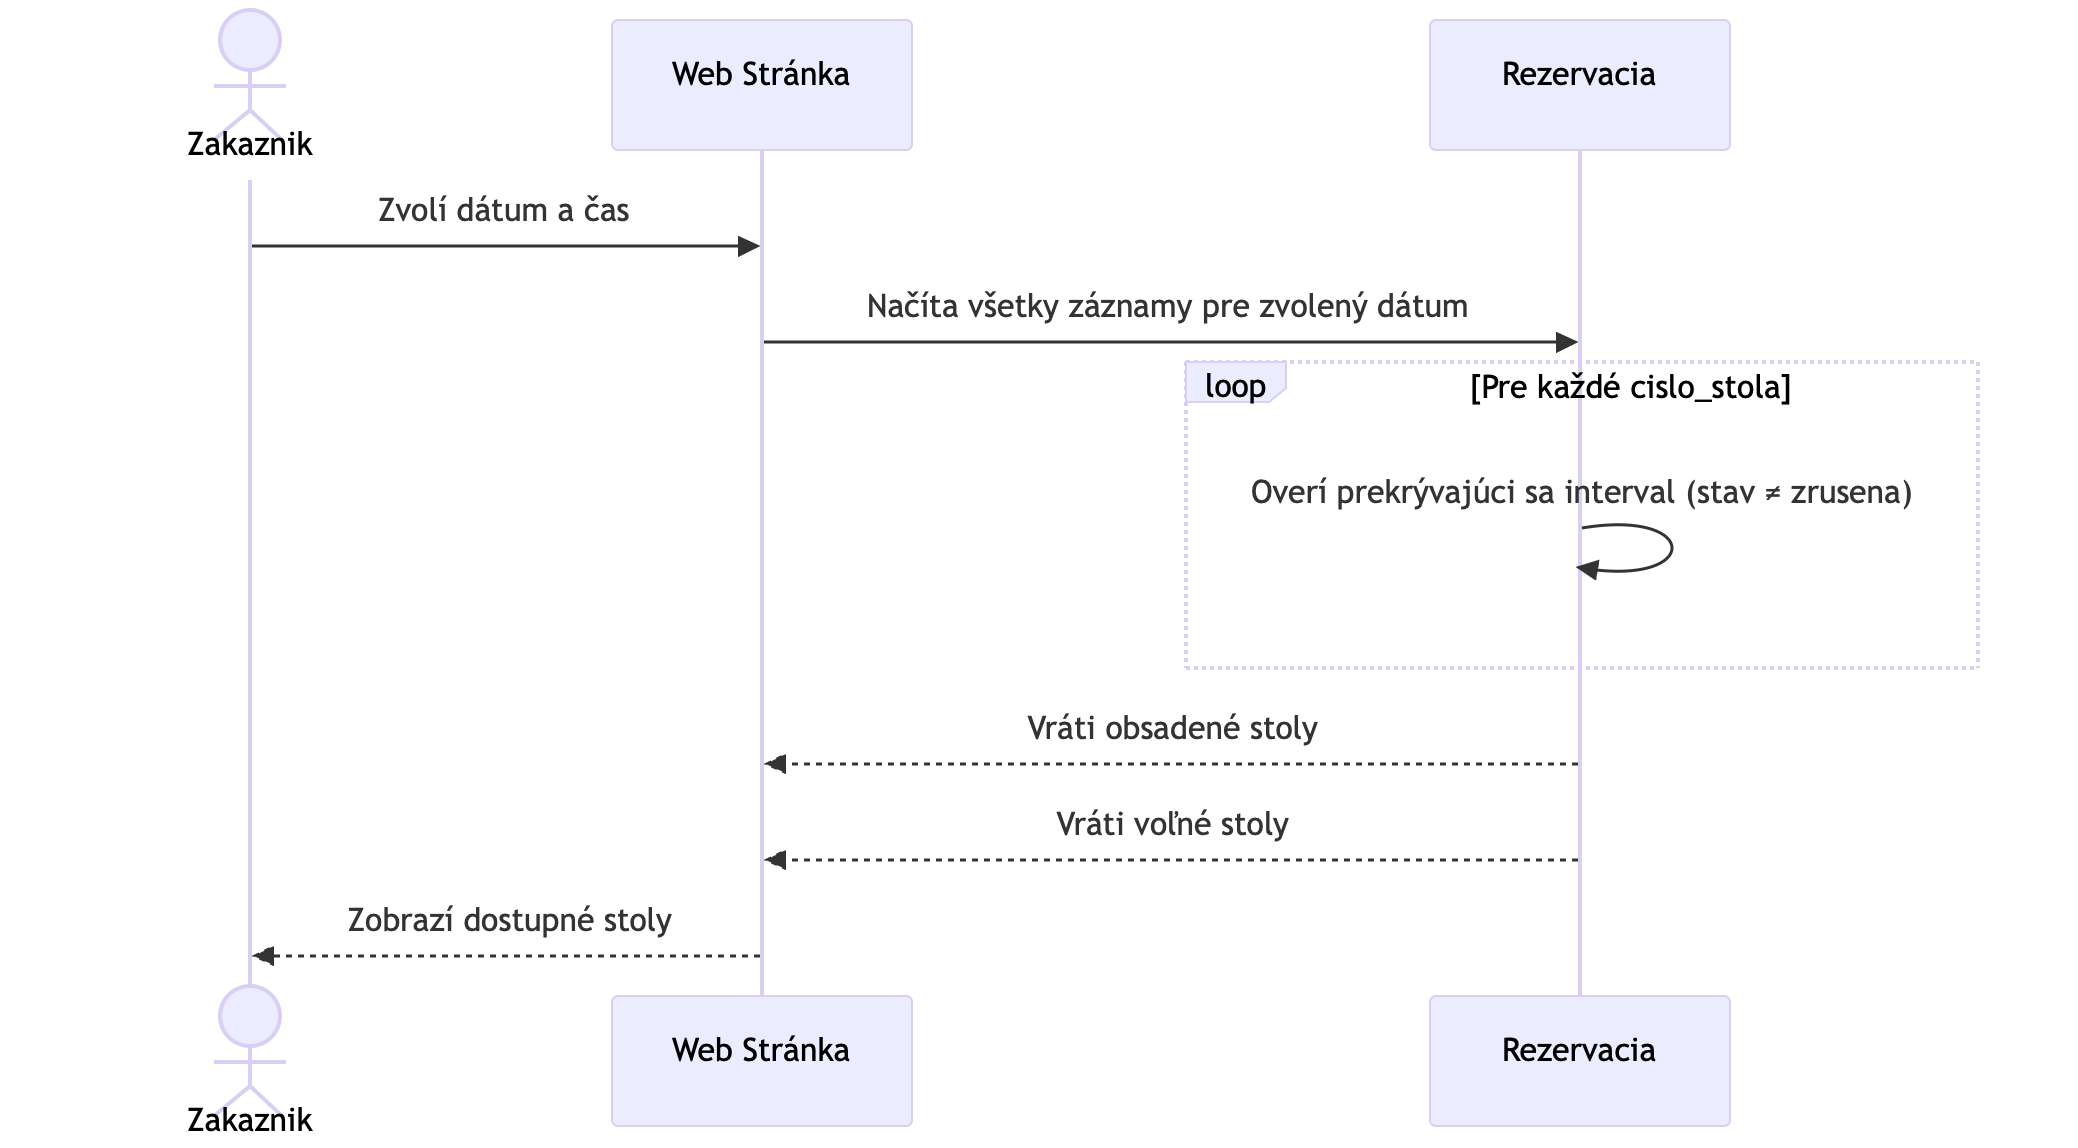
\includegraphics[width=0.75\textwidth]{../assets/diagram1cast1}
    \caption{Scenár č.1 - Časť 1: Prezeranie dostupných stolov}
    \label{fig:diagram1cast1}
\end{figure}

\begin{figure}[H]
    \centering
    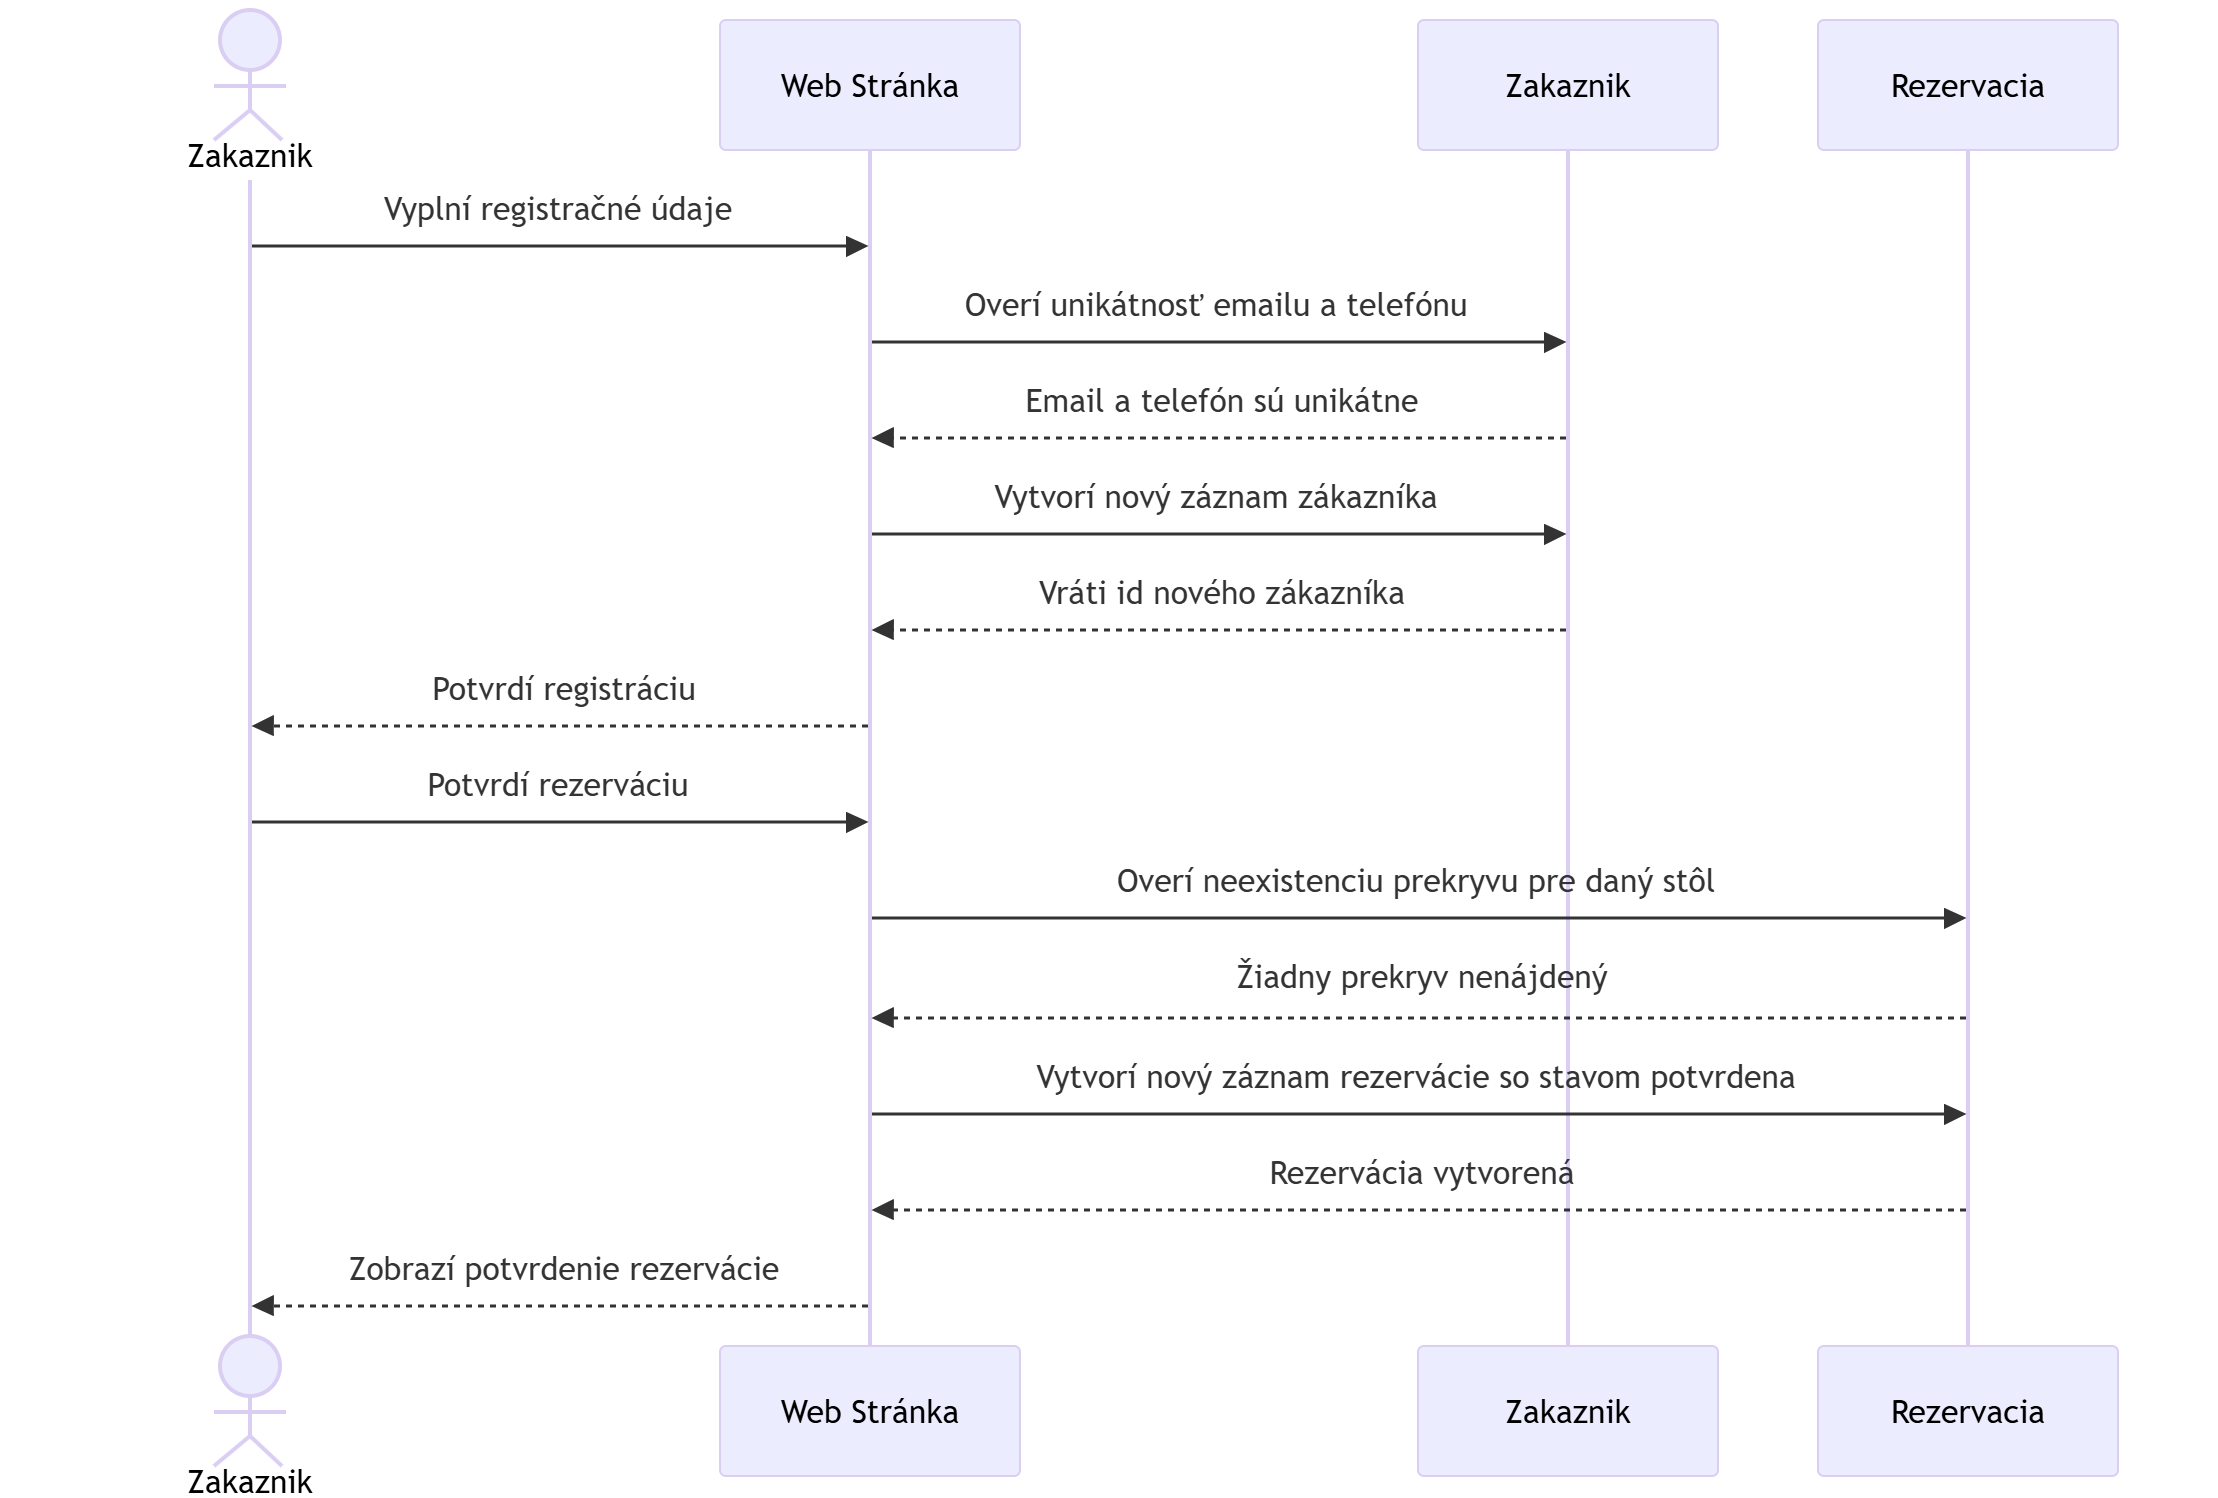
\includegraphics[width=0.75\textwidth]{../assets/diagram1cast2}
    \caption{Scenár č.1 - Časť 2: Registrácia zákazníka a vytvorenie rezervácie}
    \label{fig:diagram1cast2}
\end{figure}

\begin{figure}[H]
    \centering
    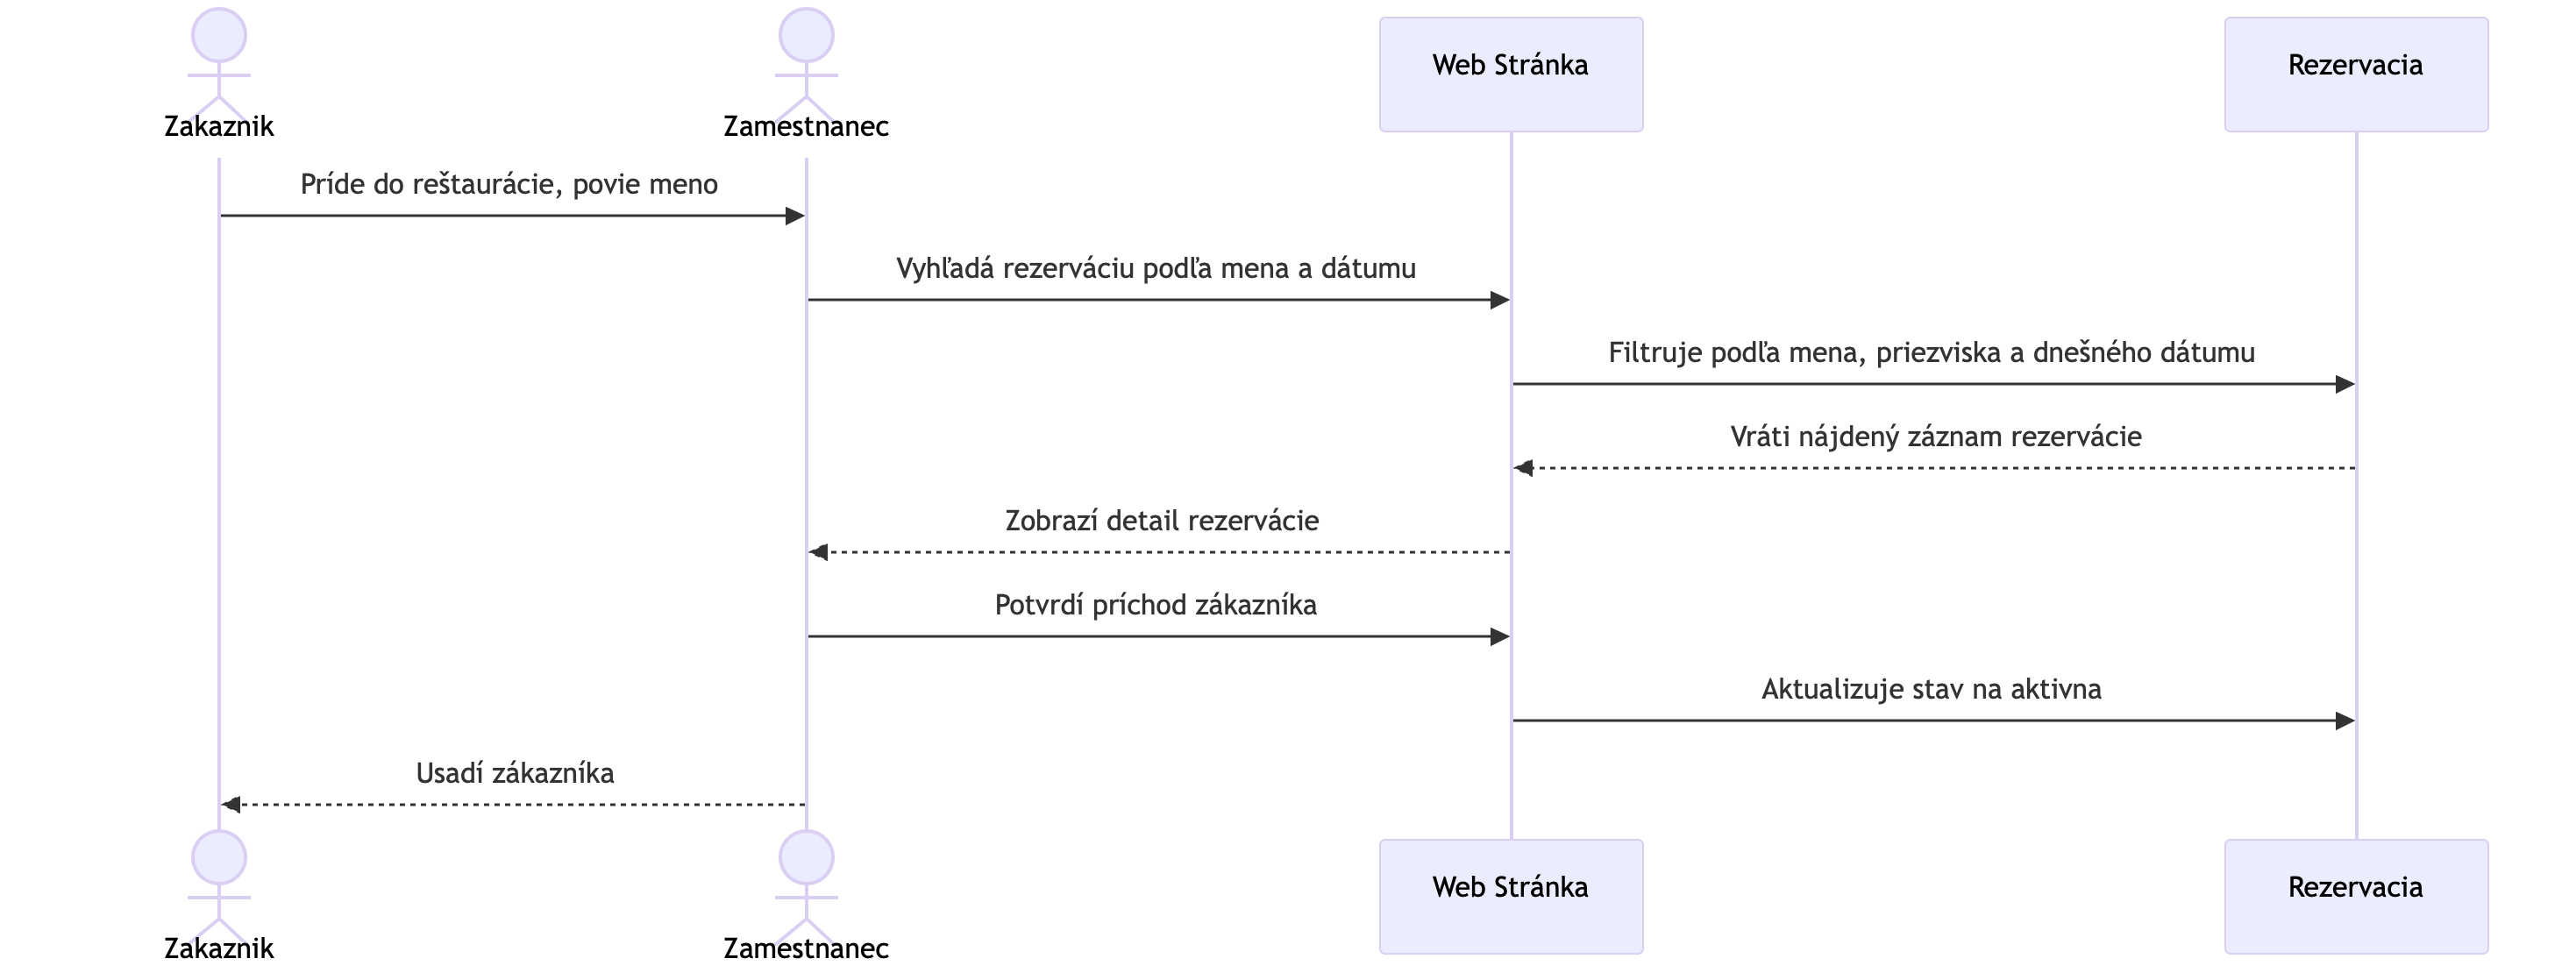
\includegraphics[width=0.95\textwidth]{../assets/diagram1cast3}
    \caption{Scenár č.1 - Časť 3: Príchod do reštaurácie}
    \label{fig:diagram1cast3}
\end{figure}

\subsubsection*{Alternatívne toky}

\begin{itemize}

    \item \textbf{Alt. A - E-mail alebo telefónne číslo už existuje (krok 2)} \\
    Overenie unikátnosti v tabuľke \texttt{Zakaznik} zlyhá. Systém informuje zákazníka, že zadaný e-mail alebo telefónne číslo je už registrované. Zákazník sa prihlási do existujúceho účtu a pokračuje krokom 3.

    \item \textbf{Alt. B - Stôl už nie je dostupný (krok 3)} \\
    Overenie v tabuľke \texttt{Rezervacia} odhalí prekrývajúci sa záznam pre daný stôl a čas. Systém informuje zákazníka a zobrazí znovu dostupné stoly. Zákazník si vyberie iný stôl alebo čas a pokračuje krokom 3.

    \item \textbf{Alt. C - Rezervácia sa nenájde (krok 4)} \\
    Prehľadávanie tabuľky \texttt{Rezervacia} prepojenej s \texttt{Zakaznik} nevráti žiadny záznam. Zamestnanec sa ospravedlní zákazníkovi. Systém prehľadá tabuľku \texttt{Stol} a vráti záznamy kde \texttt{stav = 'volny'}. Ak existuje voľný stôl, zákazník je usadený bez rezervácie a scenár končí úspešne. Ak nie, zákazník musí počkať alebo odísť.

\end{itemize}

% ─────────────────────────────────────────────────────────────────────────────

\subsection{Scenár č.2 - Objednanie jedla, platba a recenzia}

\noindent\textbf{Názov:} Objednanie jedla, platba a recenzia \\
\noindent\textbf{Popis:} Scenár pokrýva proces objednania jedla zákazníkom pri stole, spracovanie objednávky kuchyňou, doručenie jedla čašníkom, zaplatenie účtu a zanechanie recenzie. \\
\noindent\textbf{Aktér:} Zákazník, Čašník, Kuchár

\subsubsection*{Hlavný tok}

\begin{enumerate}
 
    \item \textbf{Zákazník si objedná} \\
    Zákazník si prezrie digitálne menu, vyberie položky a potvrdí objednávku. \\
    \textit{Dátová vrstva:} Prehľadáva sa tabuľka \texttt{PolozkaMenu}, vrátia sa len záznamy kde \texttt{je\_dostupna = TRUE}. Po potvrdení sa vytvorí záznam v \texttt{Objednavka} (\texttt{stav = nova}), prepojený záznam v \texttt{DineInObjednavka} s \texttt{cislo\_stola} a \texttt{id\_casnika} a pre každú vybranú položku samostatný záznam v \texttt{ObjednavkaPolozka} so \texttt{stavom = nova} a snímkou aktuálnej ceny.
 
    \item \textbf{Zákazník dostane objednávku} \\
    Zákazník sleduje stav objednávky na termináli. Keď je objednávka pripravená, čašník ju prinesie na stôl. \\
    \textit{Dátová vrstva:} Z tabuľky \texttt{Objednavka} sa načíta aktuálny \texttt{stav} podľa \texttt{id} objednávky. Žiadne záznamy sa nevytvárajú ani nemenia.
 
    \item \textbf{Zákazník zaplatí} \\
    Zákazník zvolí spôsob platby a zaplatí cez terminál pri stole. \\
    \textit{Dátová vrstva:} Systém zostaví súhrn z tabuľky \texttt{ObjednavkaPolozka} prepojenej s \texttt{PolozkaMenu} --- pre každú položku sa vráti \texttt{nazov}, \texttt{mnozstvo} a \texttt{cena\_v\_case\_objednavky}. Vytvorí sa záznam v \texttt{Faktura} s \texttt{je\_zaplatena = TRUE} a \texttt{sposob\_platby}. V \texttt{Objednavka} sa nastaví \texttt{stav = zaplatena} a v \texttt{Stol} sa nastaví \texttt{stav = volny}.
 
    \item \textbf{Zákazník zanechá recenziu} \\
    Po zaplatení systém vyzve zákazníka na hodnotenie. Zákazník zadá hodnotenie (1--5) a komentár. \\
    \textit{Dátová vrstva:} V tabuľke \texttt{Recenzia} sa vytvorí záznam s atribútmi \texttt{id\_objednavky}, \texttt{hodnotenie}, \texttt{komentar} a \texttt{cas}.
 
\end{enumerate}

\begin{figure}[H]
    \centering
    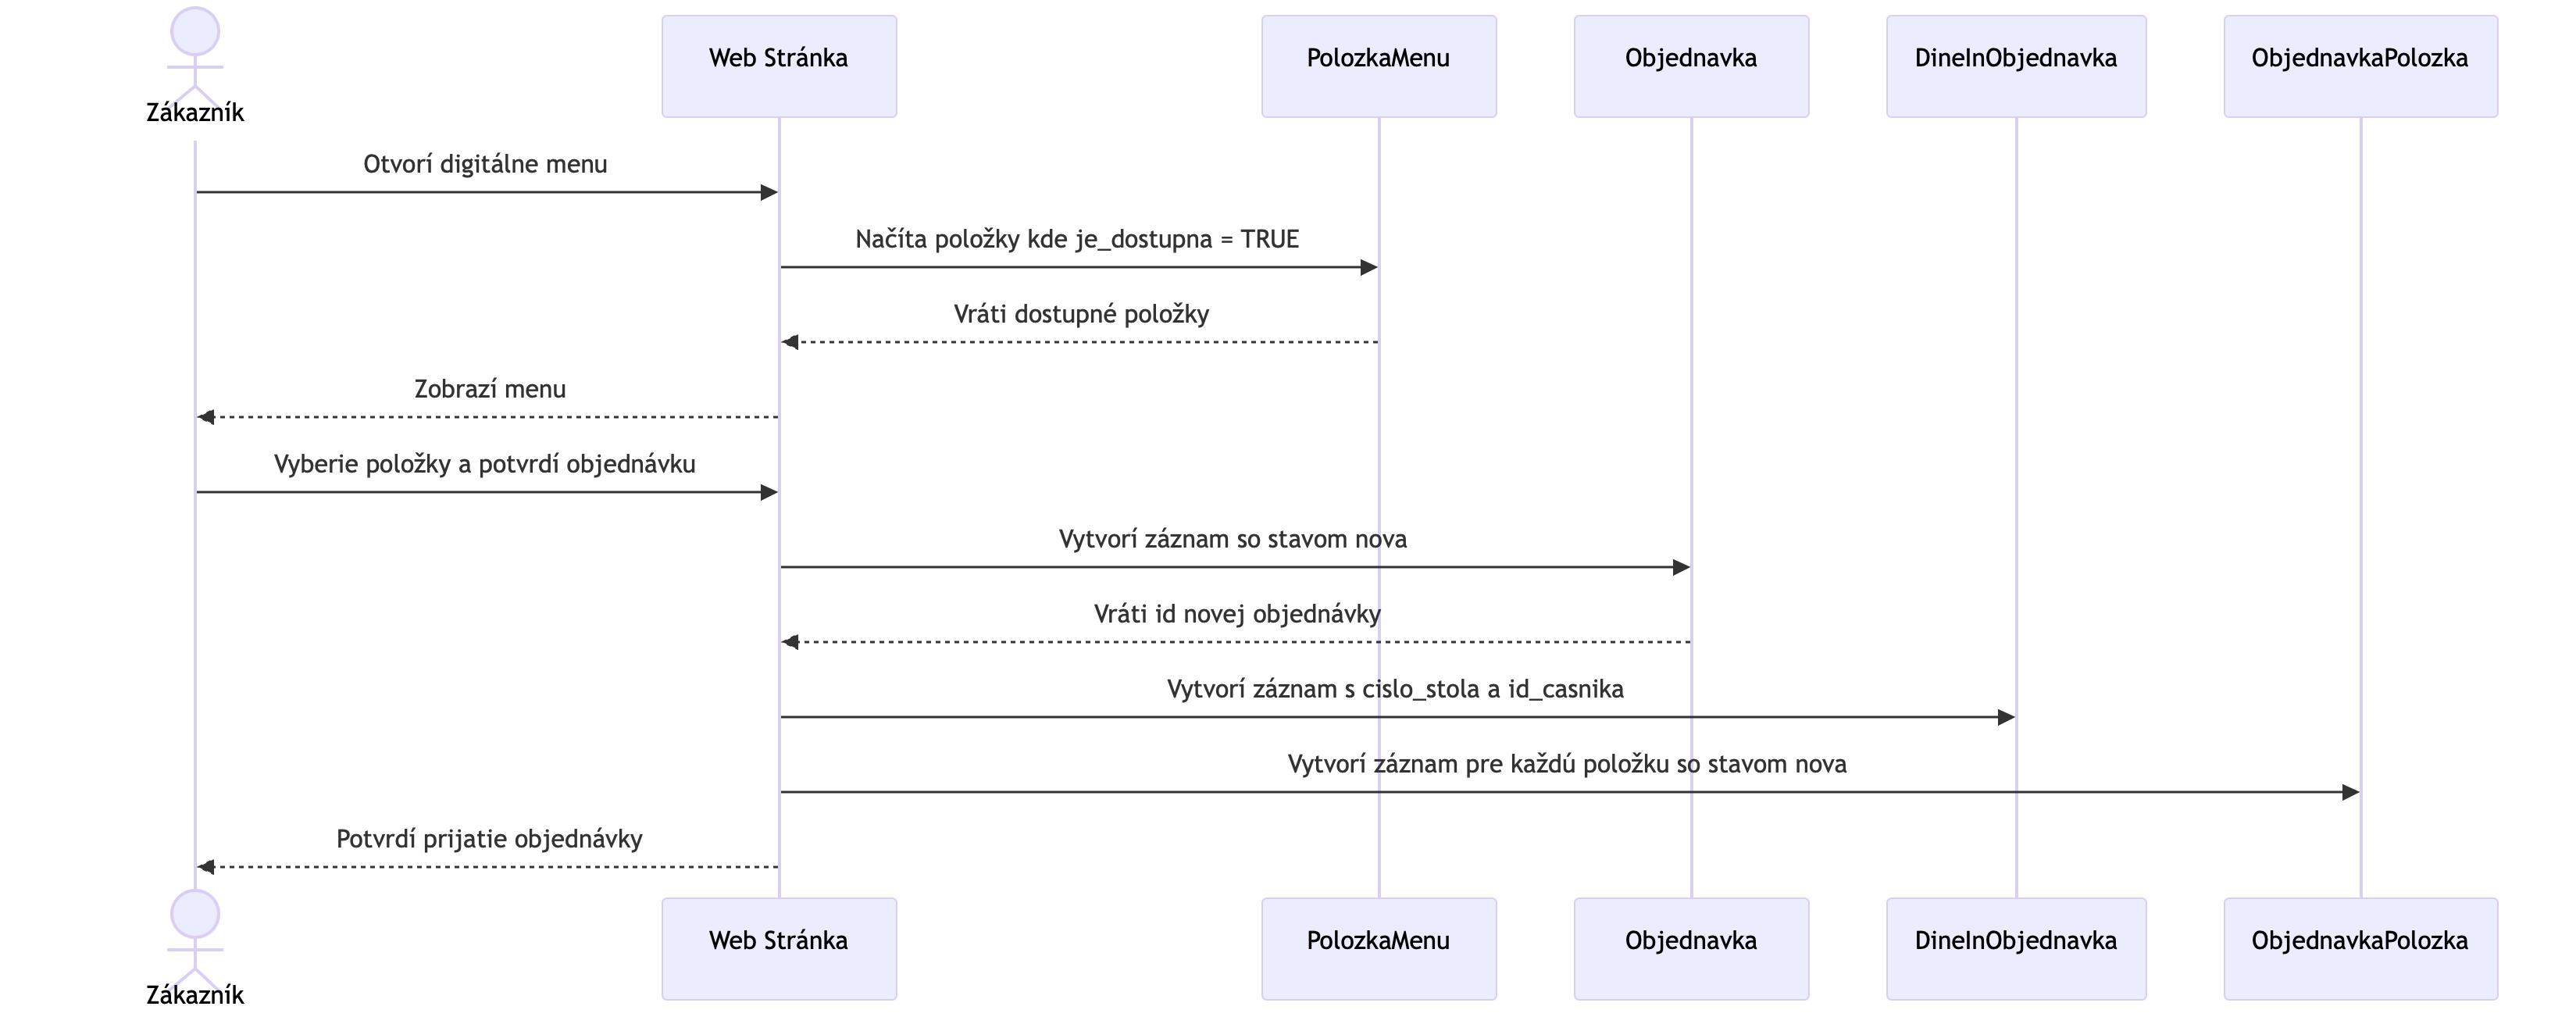
\includegraphics[width=\textwidth]{../assets/diagram2cast1}
    \caption{Scenár č.2 - Časť 1: Otvorenie menu a potvrdenie objednávky}
    \label{fig:diagram2cast1}
\end{figure}

\begin{figure}[H]
    \centering
    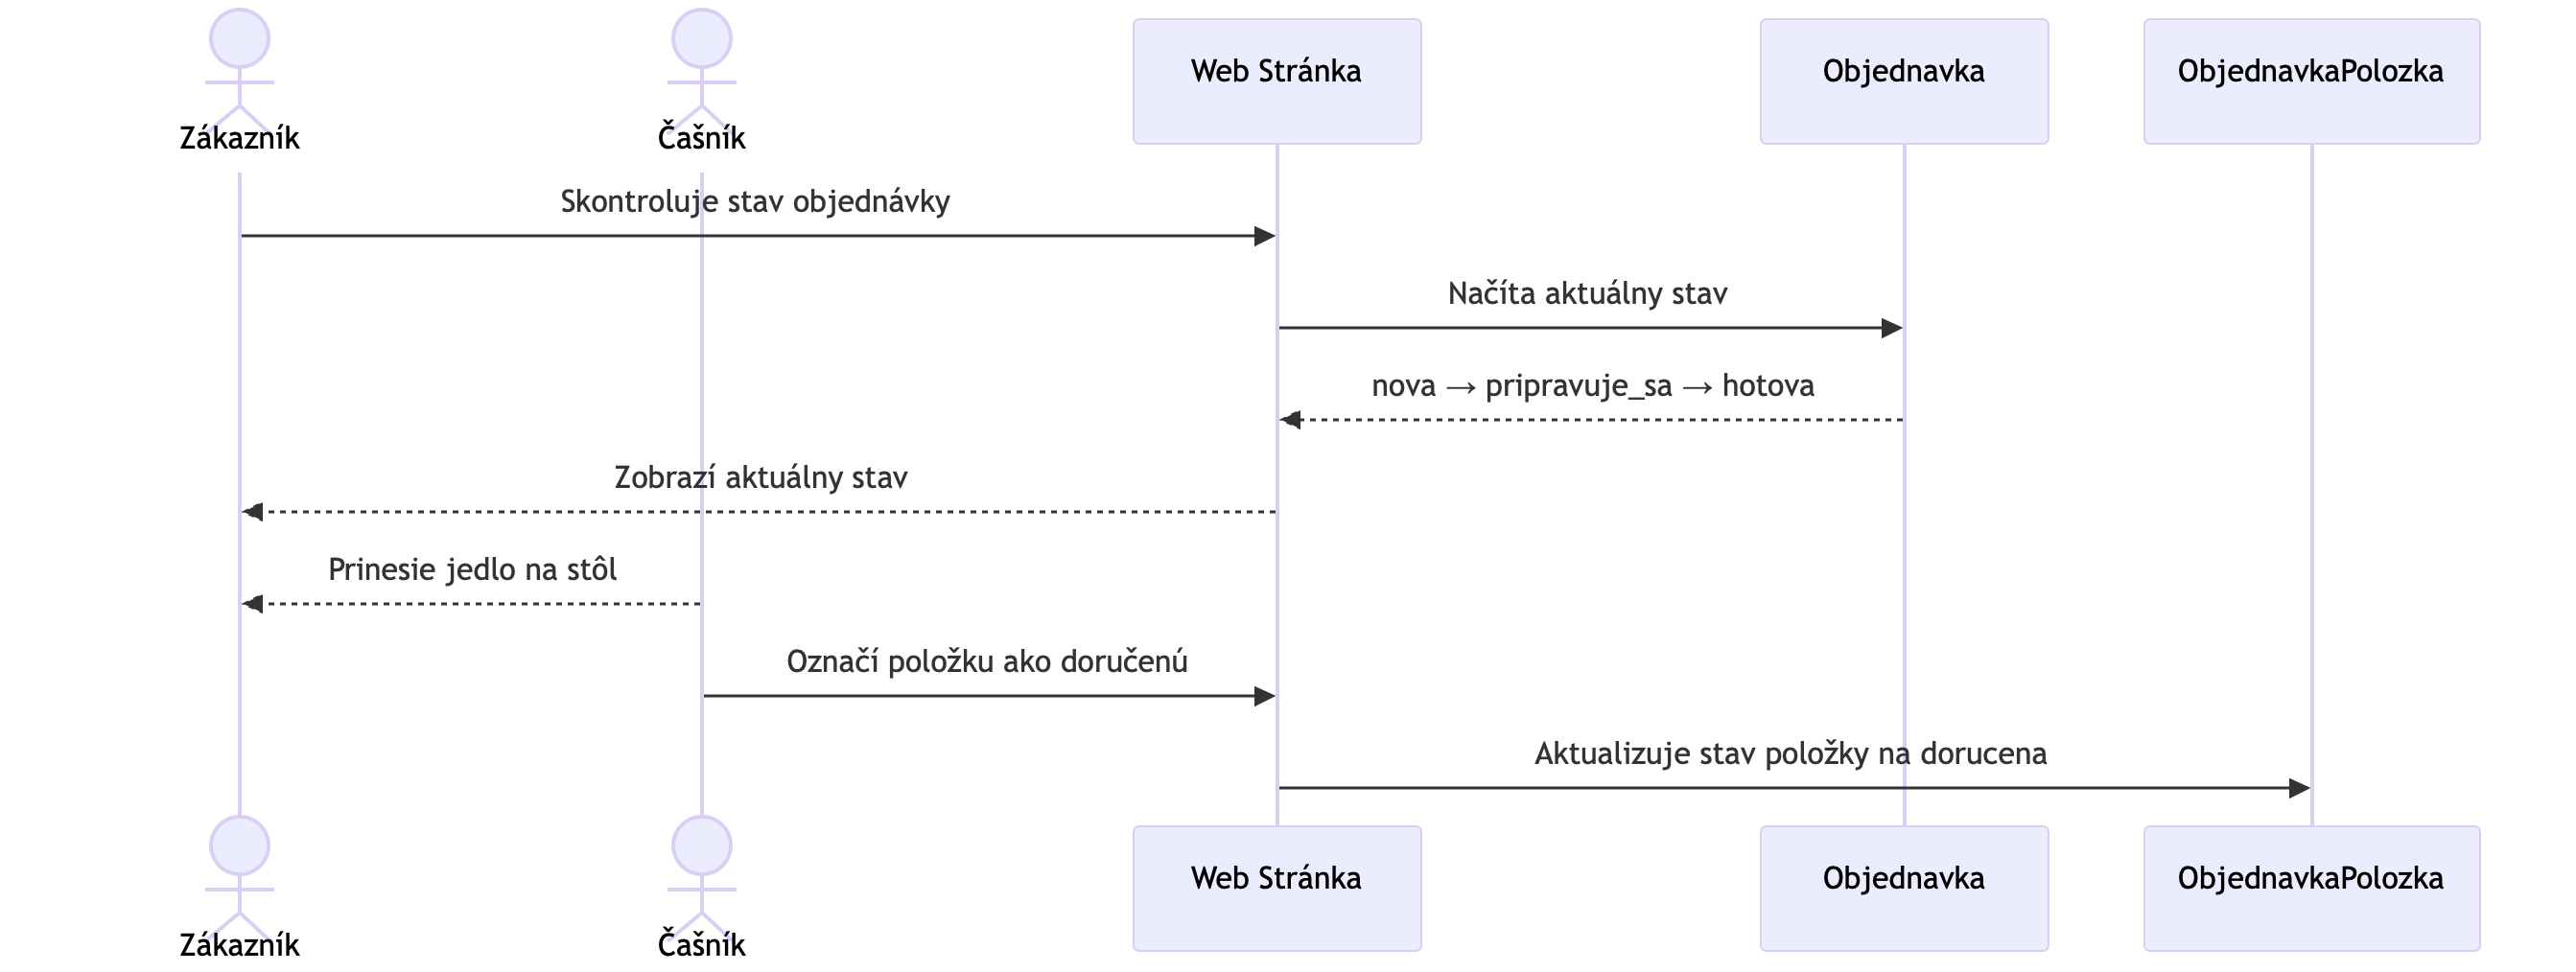
\includegraphics[width=\textwidth]{../assets/diagram2cast2}
    \caption{Scenár č.2 - Časť 2: Sledovanie stavu a doručenie jedla}
    \label{fig:diagram2cast2}
\end{figure}

\begin{figure}[H]
    \centering
    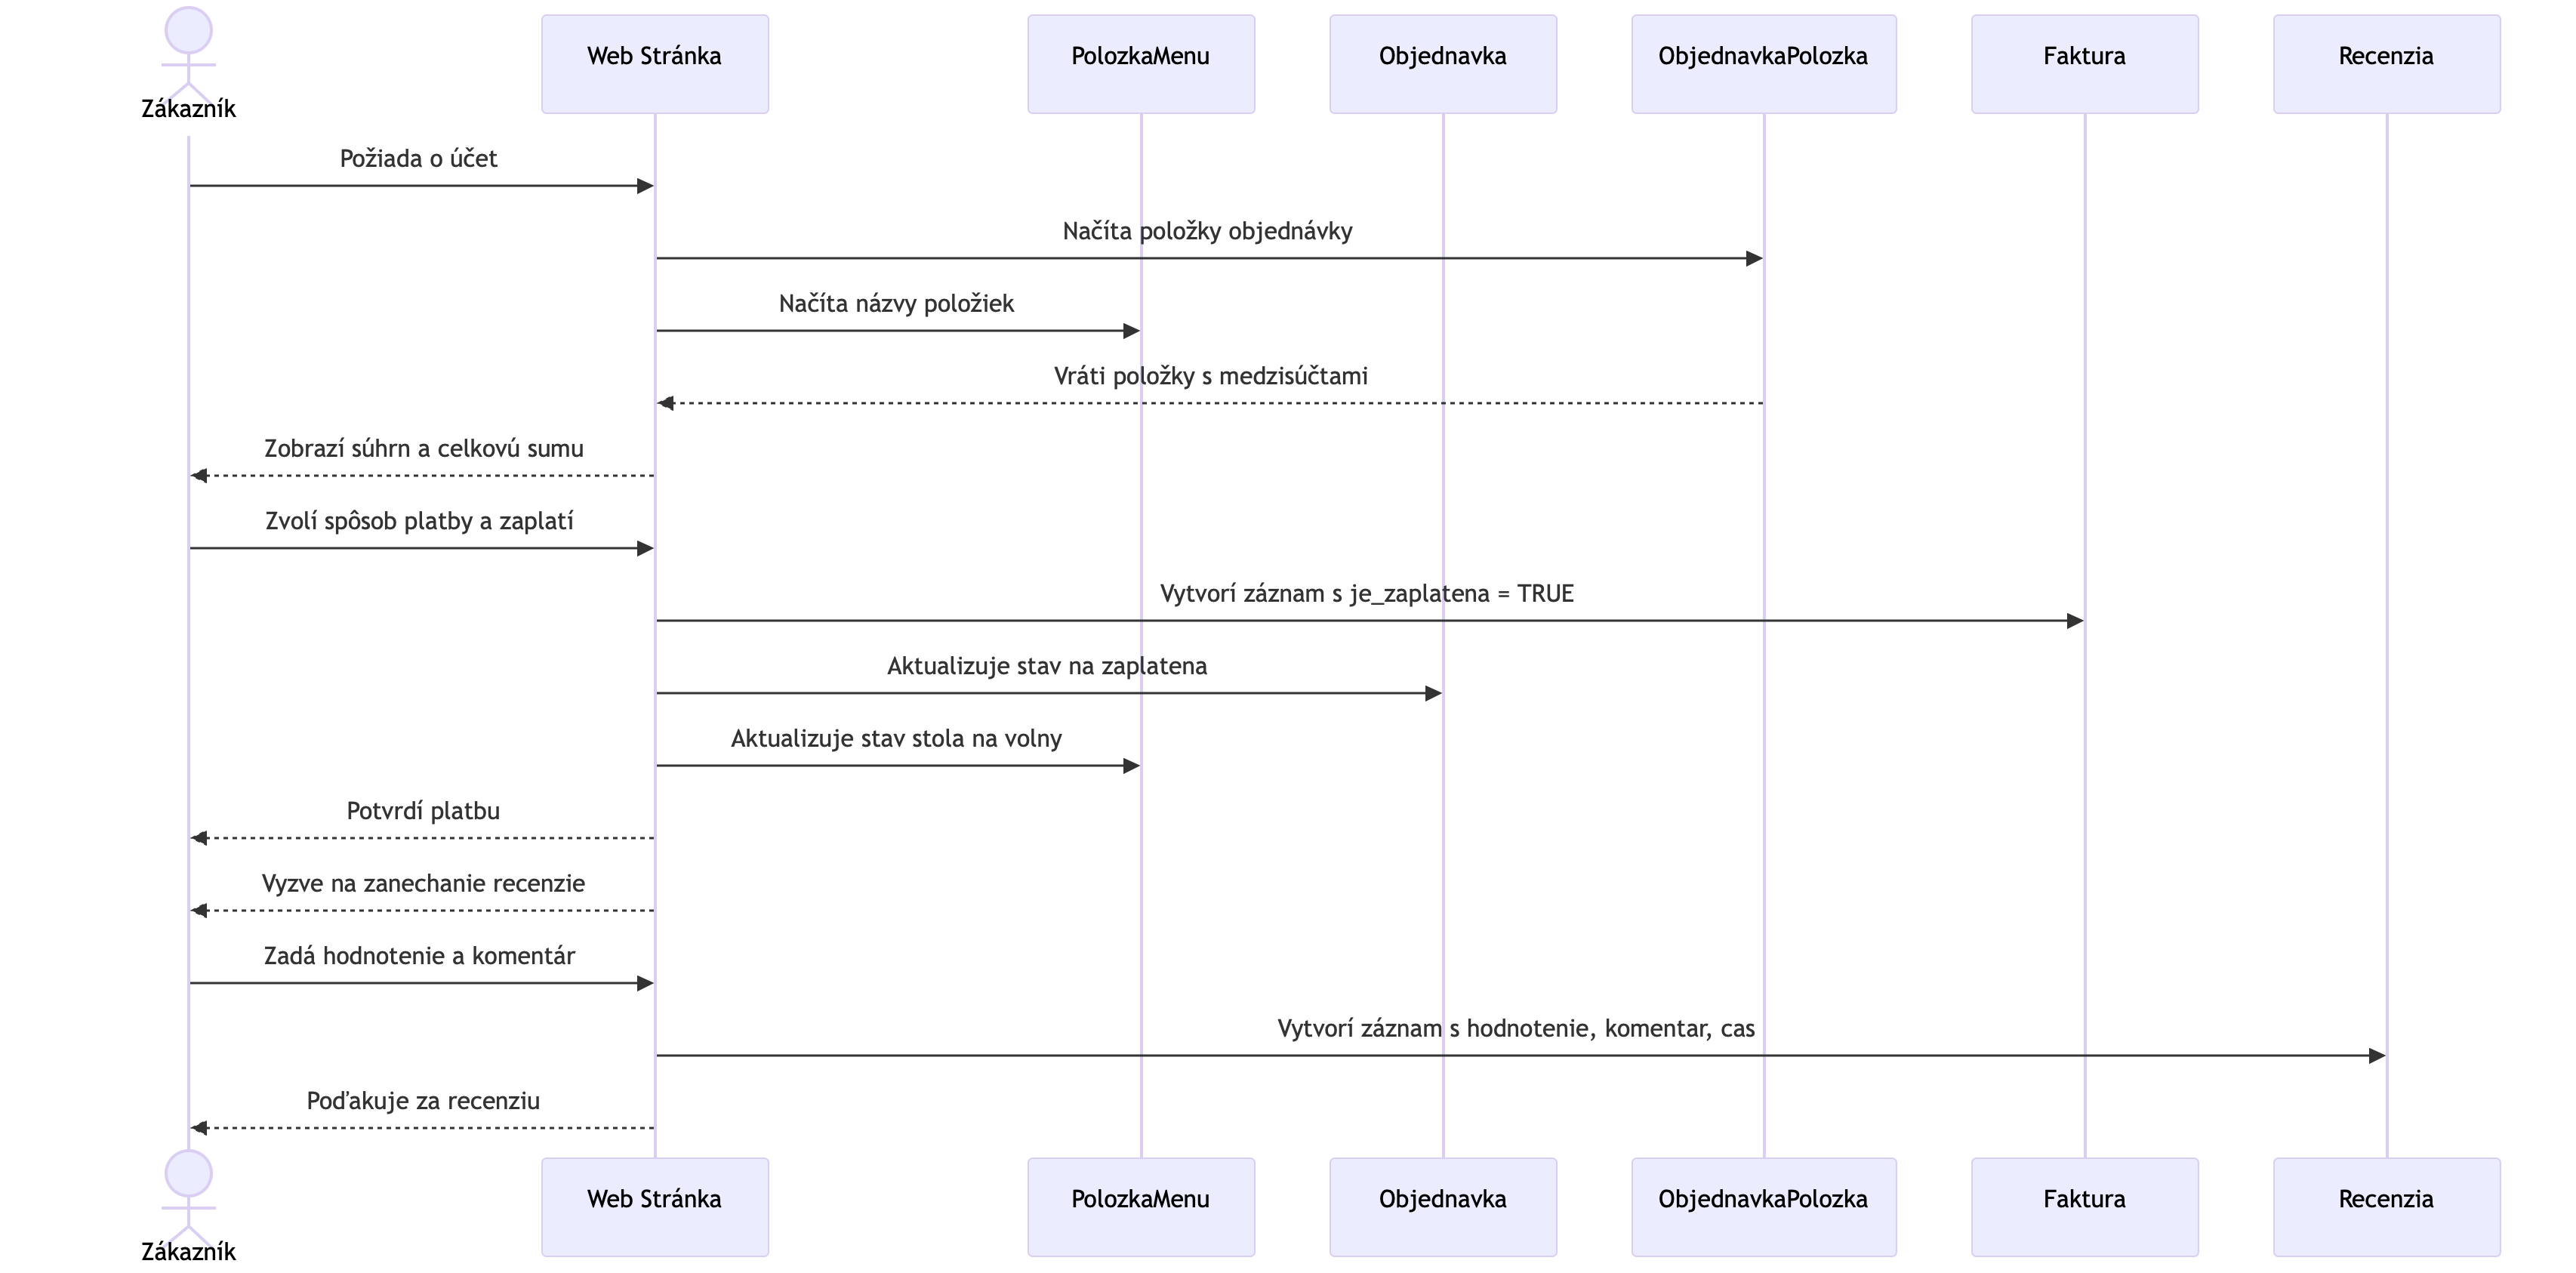
\includegraphics[width=\textwidth]{../assets/diagram2cast3}
    \caption{Scenár č.2 - Časť 3: Účet, platba a recenzia}
    \label{fig:diagram2cast3}
\end{figure}

\subsubsection*{Alternatívne toky}

\begin{itemize}

    \item \textbf{Alt. A - Položka nie je dostupná (krok 1)} \\
    Položka sa v prehľadávaní tabuľky \texttt{PolozkaMenu} nezobrazí, pretože \texttt{je\_dostupna = FALSE}. Zákazník si vyberie inú položku z menu.

    \item \textbf{Alt. B - Zákazník chce zrušiť položku (kroky 1-2)} \\
    Možné iba ak príslušný záznam v tabuľke \texttt{ObjednavkaPolozka} má atribút \texttt{stav} stále nastavený na \texttt{nova}. Aktualizuje sa \texttt{stav} daného záznamu na \texttt{zrusena}. Ak sú všetky položky zrušené, aktualizuje sa aj \texttt{stav} záznamu v tabuľke \texttt{Objednavka} na \texttt{zrusena}.

    \item \textbf{Alt. C - Zákazník nechce zanechať recenziu (krok 4)} \\
    Zákazník preskočí výzvu, žiadny záznam v tabuľke \texttt{Recenzia} sa nevytvorí. Scenár končí po kroku 3.

\end{itemize}

% ─────────────────────────────────────────────────────────────────────────────

\subsection{Scenár č.3 - Objednávka jedla s donáškou}

\noindent\textbf{Názov:} Objednávka jedla s donáškou \\
\noindent\textbf{Popis:} Scenár pokrýva proces objednania jedla cez webovú stránku s doručením domov --- od prihlásenia zákazníka a výberu položiek až po doručenie kuriérom a zanechanie recenzie. \\
\noindent\textbf{Aktér:} Zákazník, Kuriér

\subsubsection*{Hlavný tok}

\begin{enumerate}

    \item \textbf{Zákazník sa prihlási do systému} \\
    Zákazník navštívi webovú stránku a prihlási sa svojím e-mailom a heslom. \\
    \textit{Dátová vrstva:} V tabuľke \texttt{Zakaznik} sa vyhľadá záznam zodpovedajúci zadanému e-mailu a heslu. Ak záznam existuje, načítajú sa identifikačné údaje zákazníka (\texttt{id}, \texttt{meno}, \texttt{priezvisko}), ktoré sa používajú v ďalších krokoch scenára. Žiadne záznamy sa nevytvárajú ani nemenia.

    \item \textbf{Zákazník si prezrie menu a vyberie položky} \\
    Zákazník si prezrie dostupné položky, pridá ich do košíka a zadá doručovaciu adresu. \\
    \textit{Dátová vrstva:} Z tabuľky \texttt{PolozkaMenu} sa načítajú všetky dostupné položky --- pre každú sa získa \texttt{nazov}, \texttt{popis}, \texttt{aktualna\_cena} a \texttt{kategoria}. Zobrazia sa iba položky, ktoré sú označené ako dostupné. Košík je dočasne udržiavaný v pamäti aplikácie až do potvrdenia objednávky.

    \item \textbf{Zákazník potvrdí objednávku} \\
    Zákazník skontroluje obsah košíka a potvrdí objednávku s doručovacou adresou. \\
    \textit{Dátová vrstva:} Do tabuľky \texttt{Objednavka} sa vytvorí nový záznam so \texttt{stavom} nastaveným na \texttt{nova} a aktuálnym časom vytvorenia. Tento záznam slúži ako centrálny bod pre ostatné tabuľky. Do tabuľky \texttt{DeliveryObjednavka} sa vytvorí záznam prepájajúci objednávku so zákazníkom a jeho doručovacou adresou (\texttt{mesto}, \texttt{ulica}). Pole pre kuriéra zostáva prázdne a doplní sa neskôr. Pre každú položku z košíka sa do tabuľky \texttt{ObjednavkaPolozka} vytvorí samostatný záznam obsahujúci \texttt{id\_objednavky}, \texttt{id\_polozky}, \texttt{mnozstvo}, \texttt{stav} nastavený na \texttt{nova} a \texttt{cena\_v\_case\_objednavky} skopírovanú z aktuálnej ceny položky menu.

    \item \textbf{Zákazník sleduje stav objednávky} \\
    Zákazník môže priebežne kontrolovať stav svojej objednávky. \\
    \textit{Dátová vrstva:} Z tabuľky \texttt{Objednavka} sa načíta aktuálny \texttt{stav} konkrétnej objednávky identifikovanej jej \texttt{id}. Stav prechádza životným cyklom\footnote{Stavový cyklus objednávky je implementovaný ako konečný stavový automat, ktorý povoľuje len definované prechody medzi stavmi.}: \texttt{nova} $\rightarrow$ \texttt{pripravuje\_sa} $\rightarrow$ \texttt{dorucuje\_sa}. Táto operácia sa môže opakovať viackrát, žiadne záznamy nevznikajú ani sa nemenia.

    \item \textbf{Kuriér doručí objednávku} \\
    Kuriér odovzdá objednávku zákazníkovi na adrese a potvrdí doručenie v systéme. \\
    \textit{Dátová vrstva:} V tabuľke \texttt{Objednavka} sa \texttt{stav} aktualizuje na \texttt{dorucena}, čím sa uzavrie životný cyklus objednávky. V tabuľke \texttt{DeliveryObjednavka} sa doplní \texttt{id\_kuriera} --- pole, ktoré bolo prázdne od kroku 3. Zákazník dostane notifikáciu o doručení.

    \item \textbf{Zákazník zanechá recenziu} \\
    Po doručení systém vyzve zákazníka na hodnotenie. Zákazník zadá hodnotenie (1--5) a komentár. \\
    \textit{Dátová vrstva:} V tabuľke \texttt{Recenzia} sa vytvorí nový záznam s atribútmi \texttt{id\_objednavky}, \texttt{hodnotenie}, \texttt{komentar} a \texttt{cas}.

\end{enumerate}

\begin{figure}[H]
    \centering
    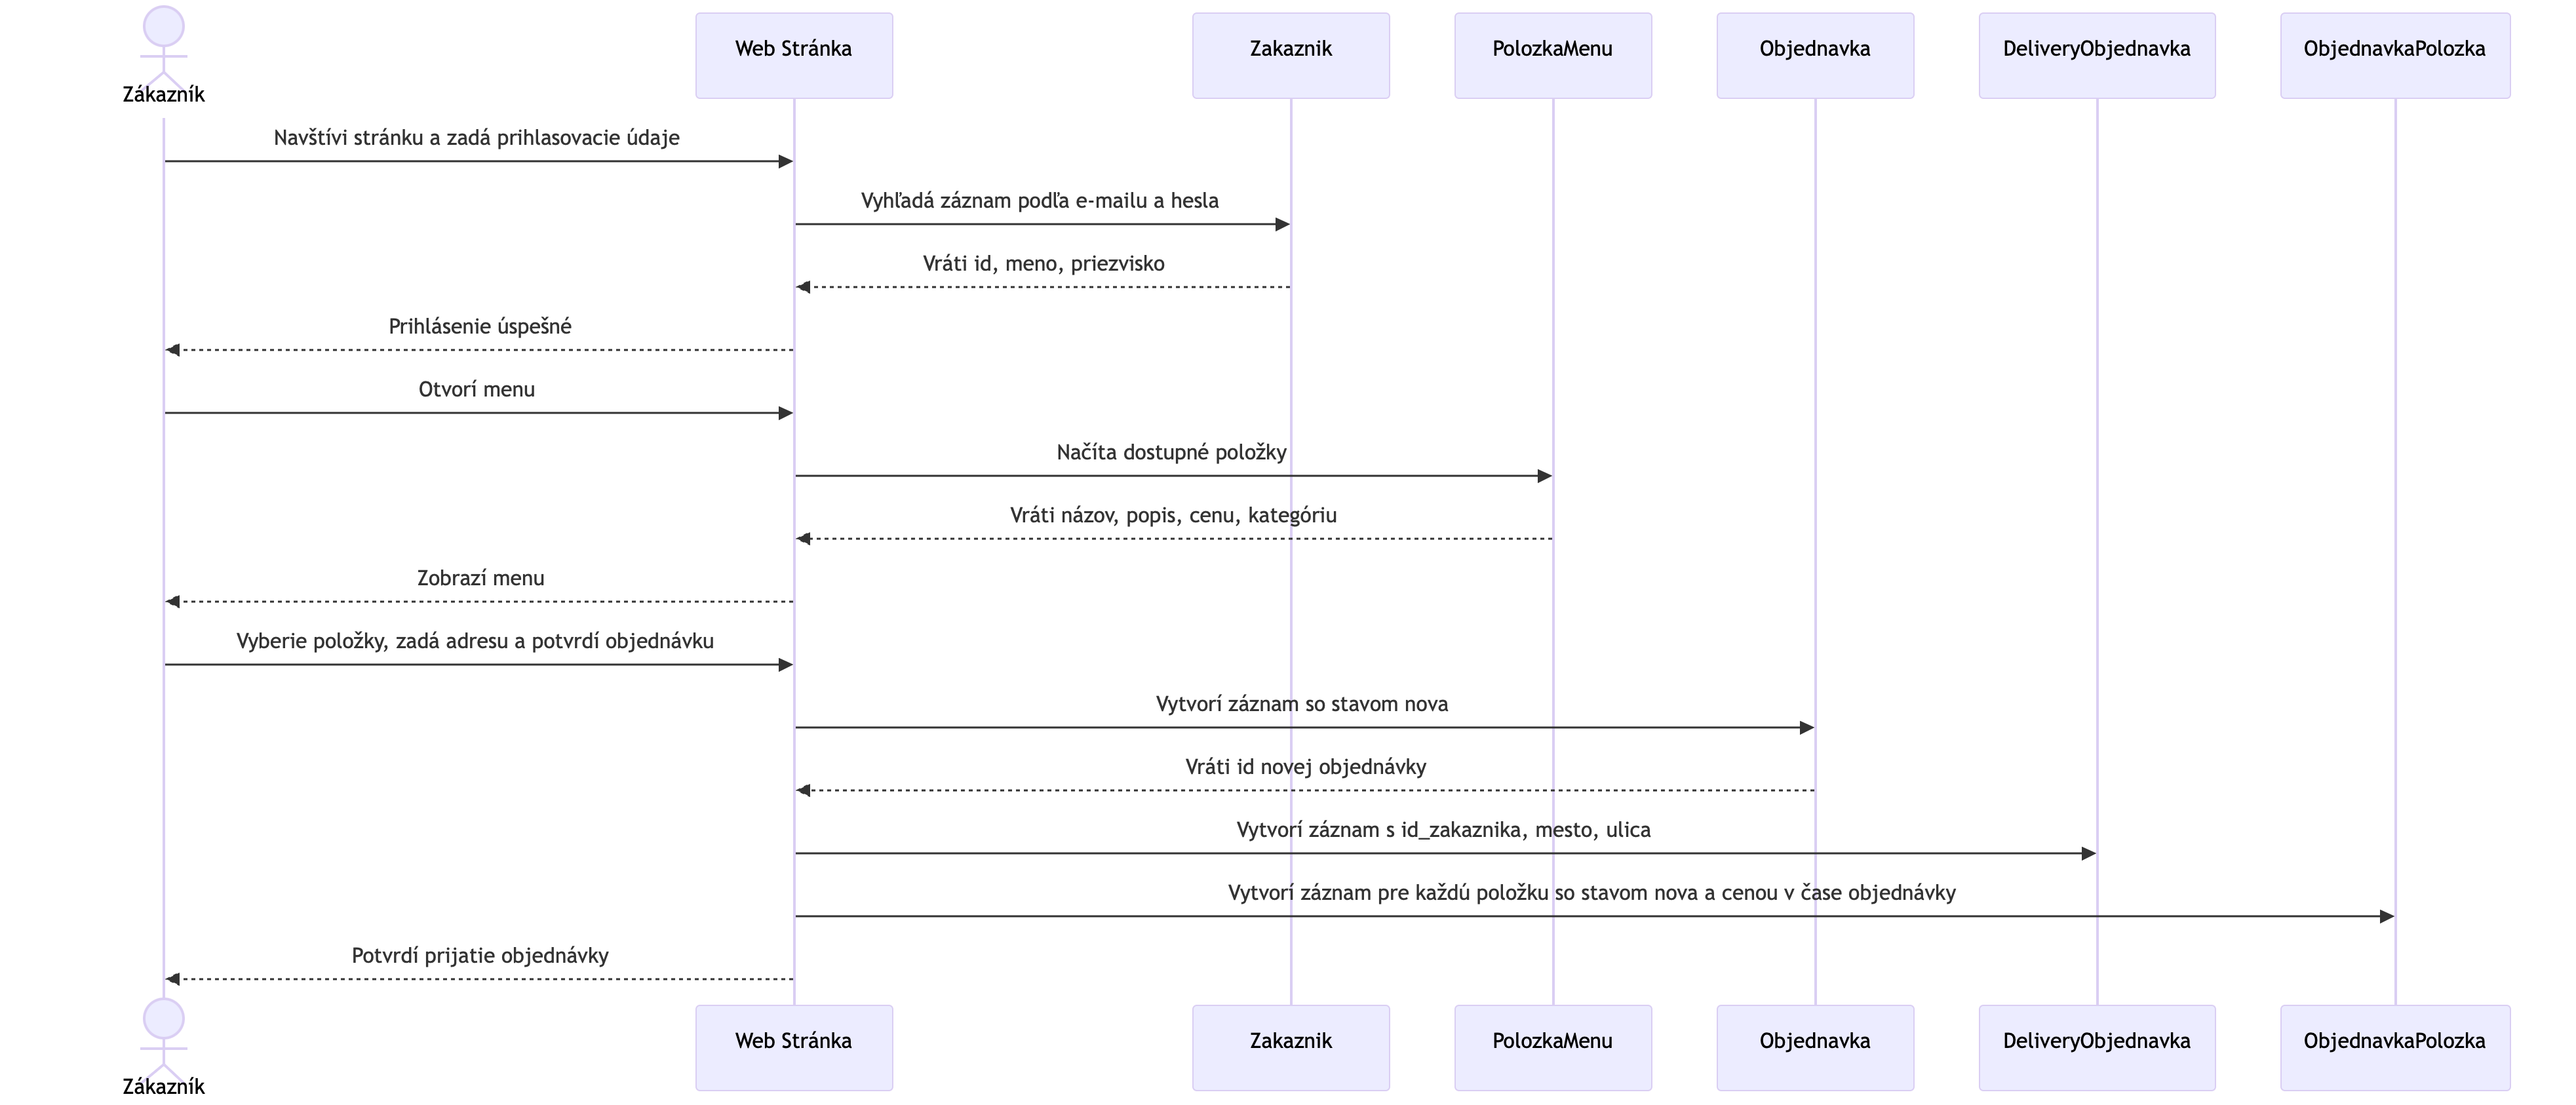
\includegraphics[width=0.85\textwidth]{../assets/diagram3cast1}
    \caption{Scenár č.3 - Časť 1: Prihlásenie, výber položiek a potvrdenie objednávky}
    \label{fig:diagram3cast1}
\end{figure}

\begin{figure}[H]
    \centering
    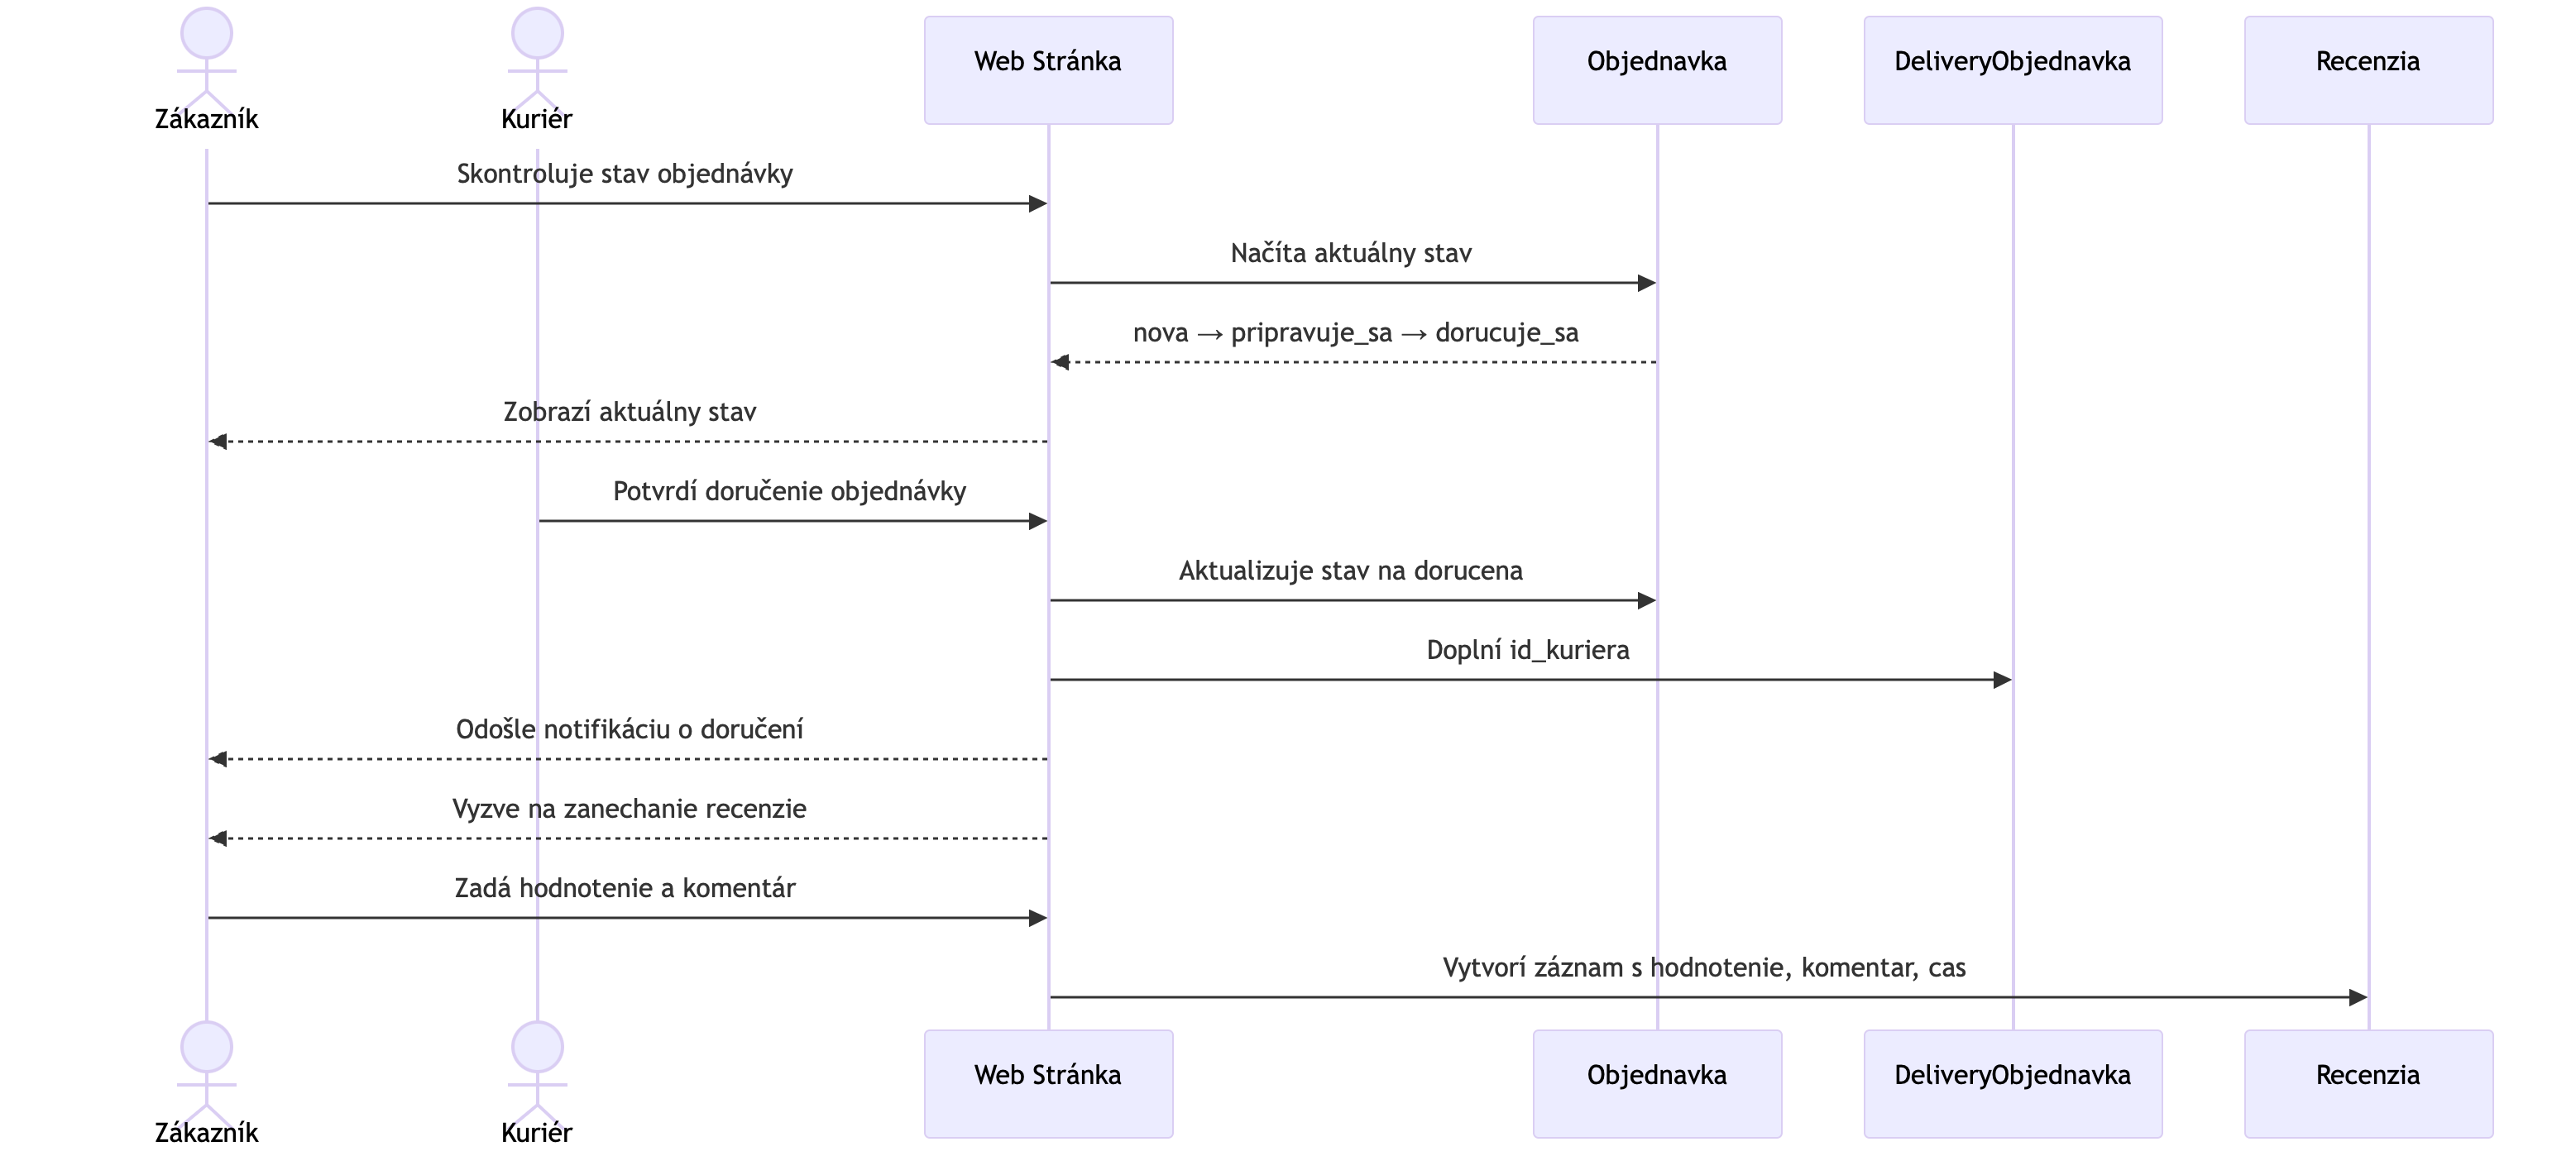
\includegraphics[width=0.85\textwidth]{../assets/diagram3cast2}
    \caption{Scenár č.3 - Časť 2: Sledovanie stavu, doručenie a recenzia}
    \label{fig:diagram3cast2}
\end{figure}

\subsubsection*{Alternatívne toky}

\begin{itemize}

    \item \textbf{Alt. A - Zákazník nie je prihlásený (krok 1)} \\
    V tabuľke \texttt{Zakaznik} sa nenájde žiadny záznam zodpovedajúci zadaným prihlasovacím údajom. Systém zobrazí chybovú hlášku „Nesprávny e-mail alebo heslo". Zákazník môže skúsiť znova alebo sa zaregistrovať.

    \item \textbf{Alt. B - Položka nie je dostupná (krok 2)} \\
    Položky s príznakom nedostupnosti sa pri načítaní tabuľky \texttt{PolozkaMenu} jednoducho nezobrazia. Zákazník si vyberie inú položku z menu.

    \item \textbf{Alt. C - Zákazník zruší objednávku (kroky 3--4)} \\
    Zrušenie je možné iba ak \texttt{stav} záznamu v tabuľke \texttt{Objednavka} je ešte \texttt{nova}. V tabuľke \texttt{Objednavka} sa \texttt{stav} zmení na \texttt{zrusena}. V tabuľke \texttt{ObjednavkaPolozka} sa \texttt{stav} zmení na \texttt{zrusena} pre všetky položky danej objednávky. Záznamy sa nevymažú\footnote{Namiesto fyzického vymazania sa používa logické zrušenie záznamu, aby bola zachovaná auditná stopa a historické dáta.} --- zachováva sa história.

    \item \textbf{Alt. D - Zákazník nechce zanechať recenziu (krok 6)} \\
    Zákazník preskočí výzvu, žiadny záznam v tabuľke \texttt{Recenzia} sa nevytvorí. Scenár končí po kroku 5.

\end{itemize}

% ─────────────────────────────────────────────────────────────────────────────

\newpage
\subsection{Scenár č.4 - Príprava a výdaj jedla zamestnancami}

\noindent\textbf{Názov:} Príprava a výdaj jedla zamestnancami \\
\noindent\textbf{Popis:} Scenár pokrýva proces spracovania objednávky zo strany kuchyne a čašníka --- od zobrazenia novej objednávky kuchárovi, cez jej prípravu, až po fyzické doručenie jedla zákazníkovi čašníkom. \\
\noindent\textbf{Aktér:} Kuchár, Čašník, Zákazník\footnotemark
\footnotetext{Zákazník nie je priamym aktérom scenára, vystupuje iba ako vedľajší účastník procesu.}

\subsubsection*{Hlavný tok}

\begin{enumerate}

    \item \textbf{Kuchár uvidí novú objednávku} \\
    Po potvrdení objednávky zákazníkom sa táto automaticky zobrazí v kuchynskom systéme. \\
    \textit{Dátová vrstva:} Z tabuľky \texttt{Objednavka} sa načítajú všetky záznamy so \texttt{stavom = nova}, prepojené s tabuľkou \texttt{ObjednavkaPolozka} cez \texttt{id\_objednavky}. Pre každú položku sa získa \texttt{id\_polozky} a \texttt{mnozstvo}. Kuchár vidí zoznam položiek bez osobných údajov zákazníka.

    \item \textbf{Kuchár prevezme objednávku} \\
    Kuchár označí objednávku ako prevzatú a začne s prípravou. \\
    \textit{Dátová vrstva:} V tabuľke \texttt{Objednavka} sa \texttt{stav} aktualizuje na \texttt{pripravuje\_sa}. Ostatní kuchári vidia, že objednávka je už spracovávaná.

    \item \textbf{Kuchár dokončí prípravu} \\
    Po dokončení prípravy všetkých položiek kuchár označí objednávku ako hotovú. \\
    \textit{Dátová vrstva:} V tabuľke \texttt{Objednavka} sa \texttt{stav} aktualizuje na \texttt{hotova}. Systém notifikuje čašníka priradeného k danému stolu.

    \item \textbf{Čašník doručí jedlo zákazníkovi} \\
    Čašník si v systéme skontroluje, ktoré objednávky sú hotové a prinesie ich k príslušnému stolu. \\
    \textit{Dátová vrstva:} Z tabuľky \texttt{Objednavka} sa načítajú záznamy so \texttt{stavom = hotova} prepojené s tabuľkou \texttt{DineInObjednavka} cez \texttt{id\_objednavky}, aby čašník vedel číslo stola. Po doručení každej položky čašník aktualizuje \texttt{stav} príslušného záznamu v tabuľke \texttt{ObjednavkaPolozka} na \texttt{dorucena}.

\end{enumerate}

\begin{figure}[H]
    \centering
    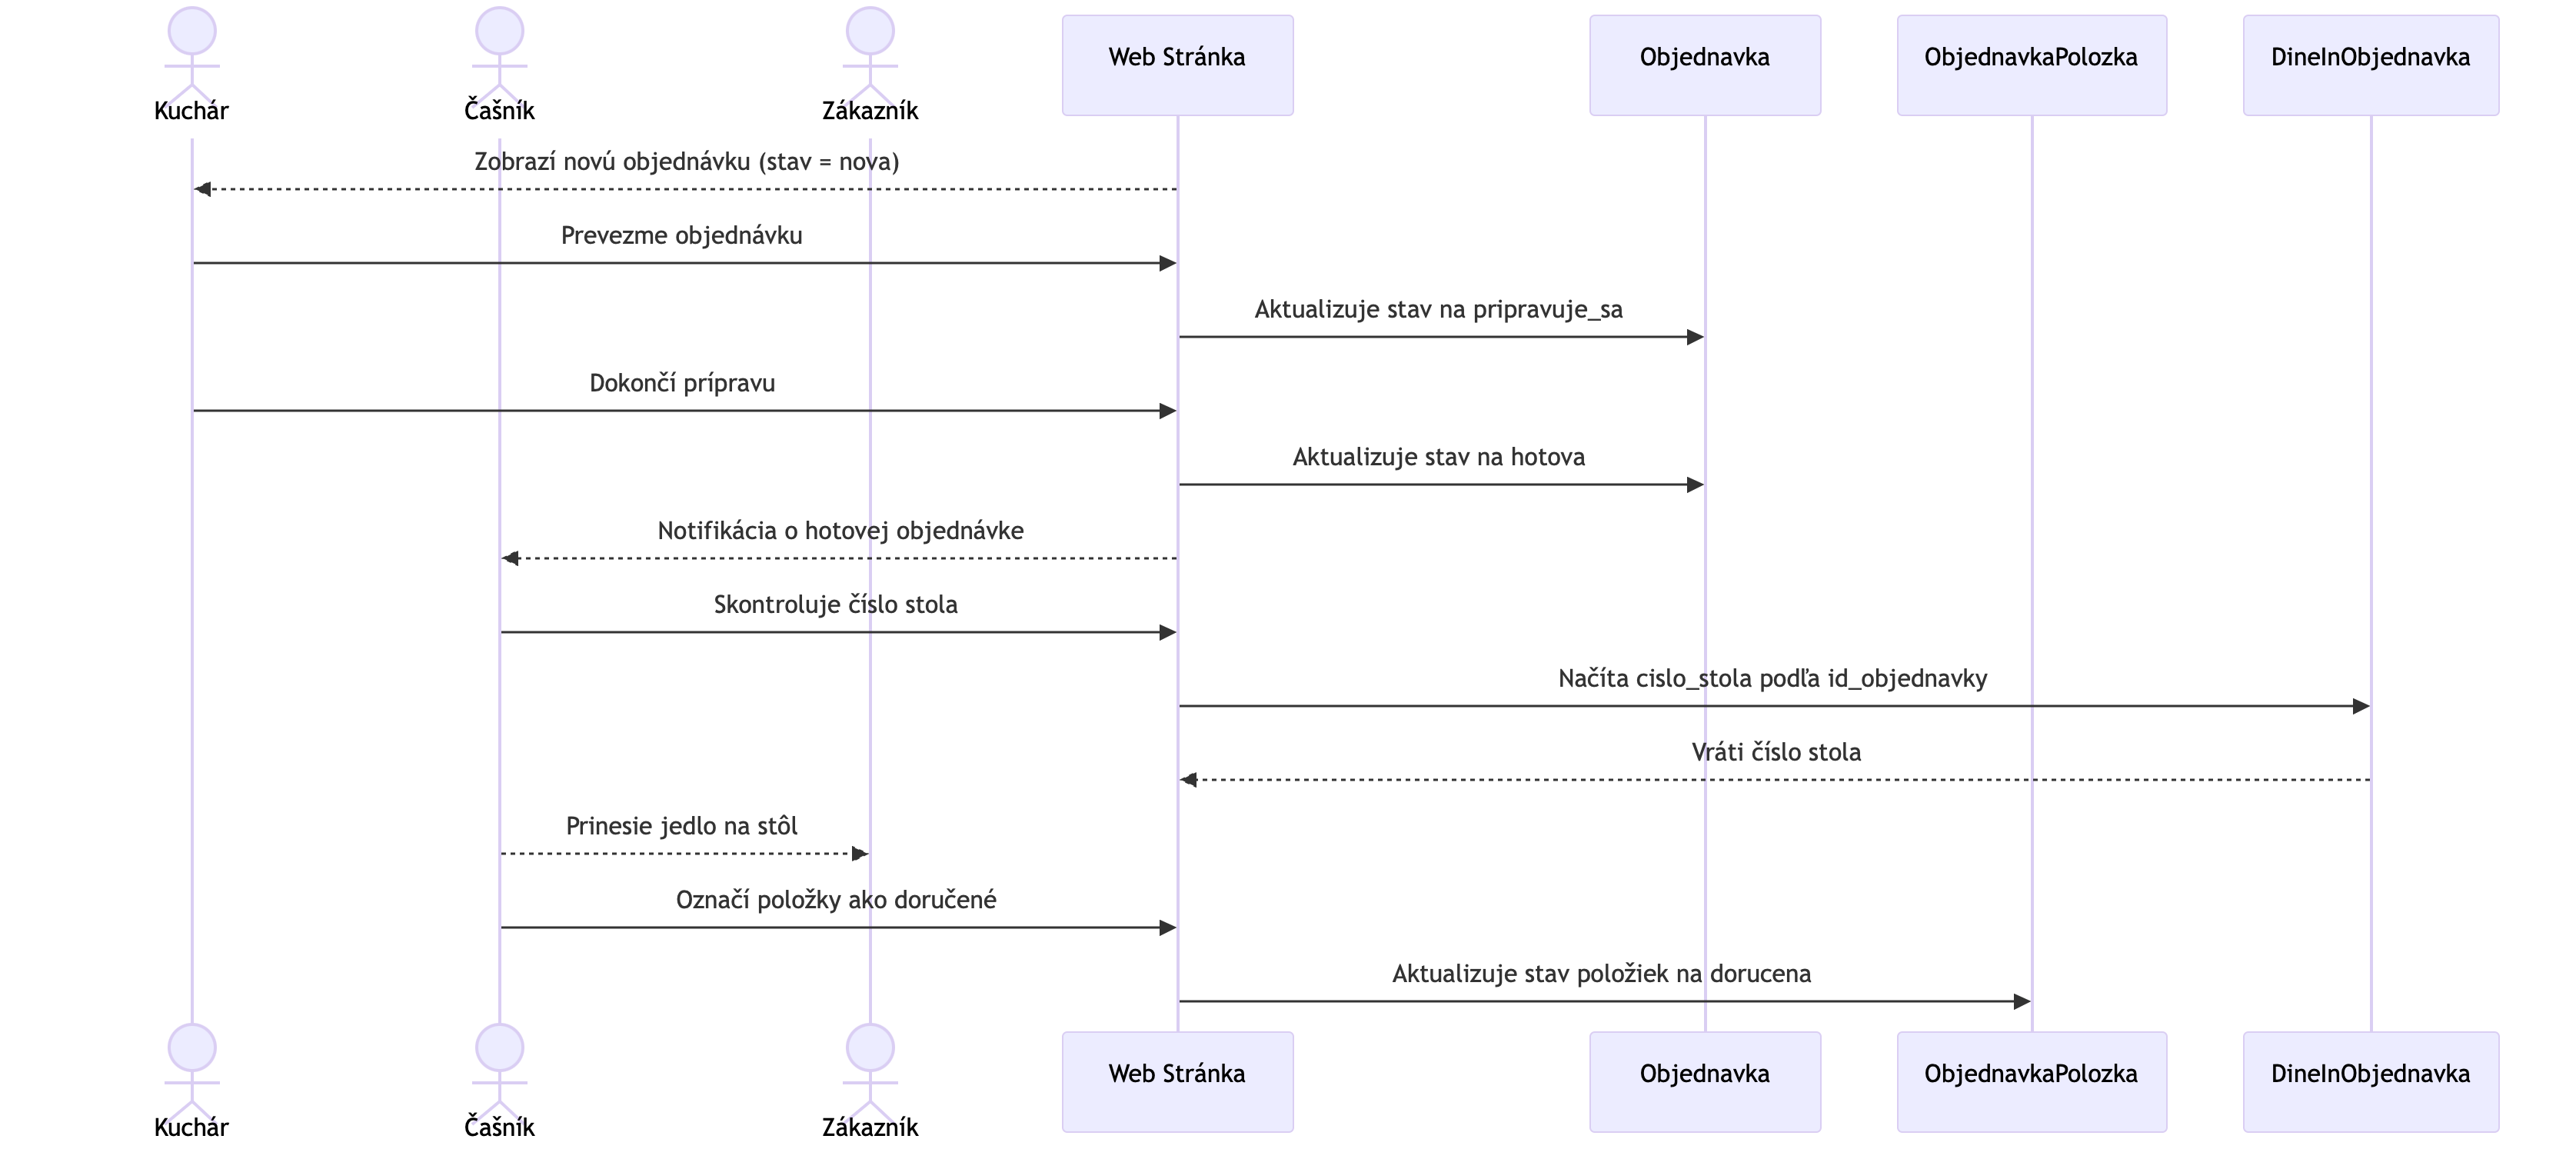
\includegraphics[width=\textwidth]{../assets/diagram4cast1}
    \caption{Scenár č.4 - Príprava objednávky kuchárom a výdaj čašníkom}
    \label{fig:diagram4cast1}
\end{figure}

\subsubsection*{Alternatívne toky}

\begin{itemize}

    \item \textbf{Alt. A - Položka nie je možné pripraviť (krok 2)} \\
    Kuchár zistí, že niektorú položku nie je možné pripraviť (napr. došla surovina). V tabuľke \texttt{ObjednavkaPolozka} sa \texttt{stav} danej položky zmení na \texttt{zrusena}. Ak sú zrušené všetky položky, aktualizuje sa aj \texttt{stav} záznamu v tabuľke \texttt{Objednavka} na \texttt{zrusena}. Čašník informuje zákazníka.

    \item \textbf{Alt. B - Čašník nenájde zákazníka pri stole (krok 4)} \\
    Pri doručení čašník zistí, že stôl je prázdny. Položky zostávajú v stave \texttt{hotova} v tabuľke \texttt{ObjednavkaPolozka}. Čašník situáciu rieši manuálne --- buď počká, alebo eskaluje na manažéra.

\end{itemize}

\newpage
\section{Návrh relačného modelu}
\label{sec:rm_design}

\newpage
\section{Zhodnotenie}
\label{sec:conclusion}

\newpage
\appendix

\section{Prílohy}
\label{sec:attachments}

% ─── Scenár 1 ─────────────────────────────────────

\begin{figure}[H]
    \centering
    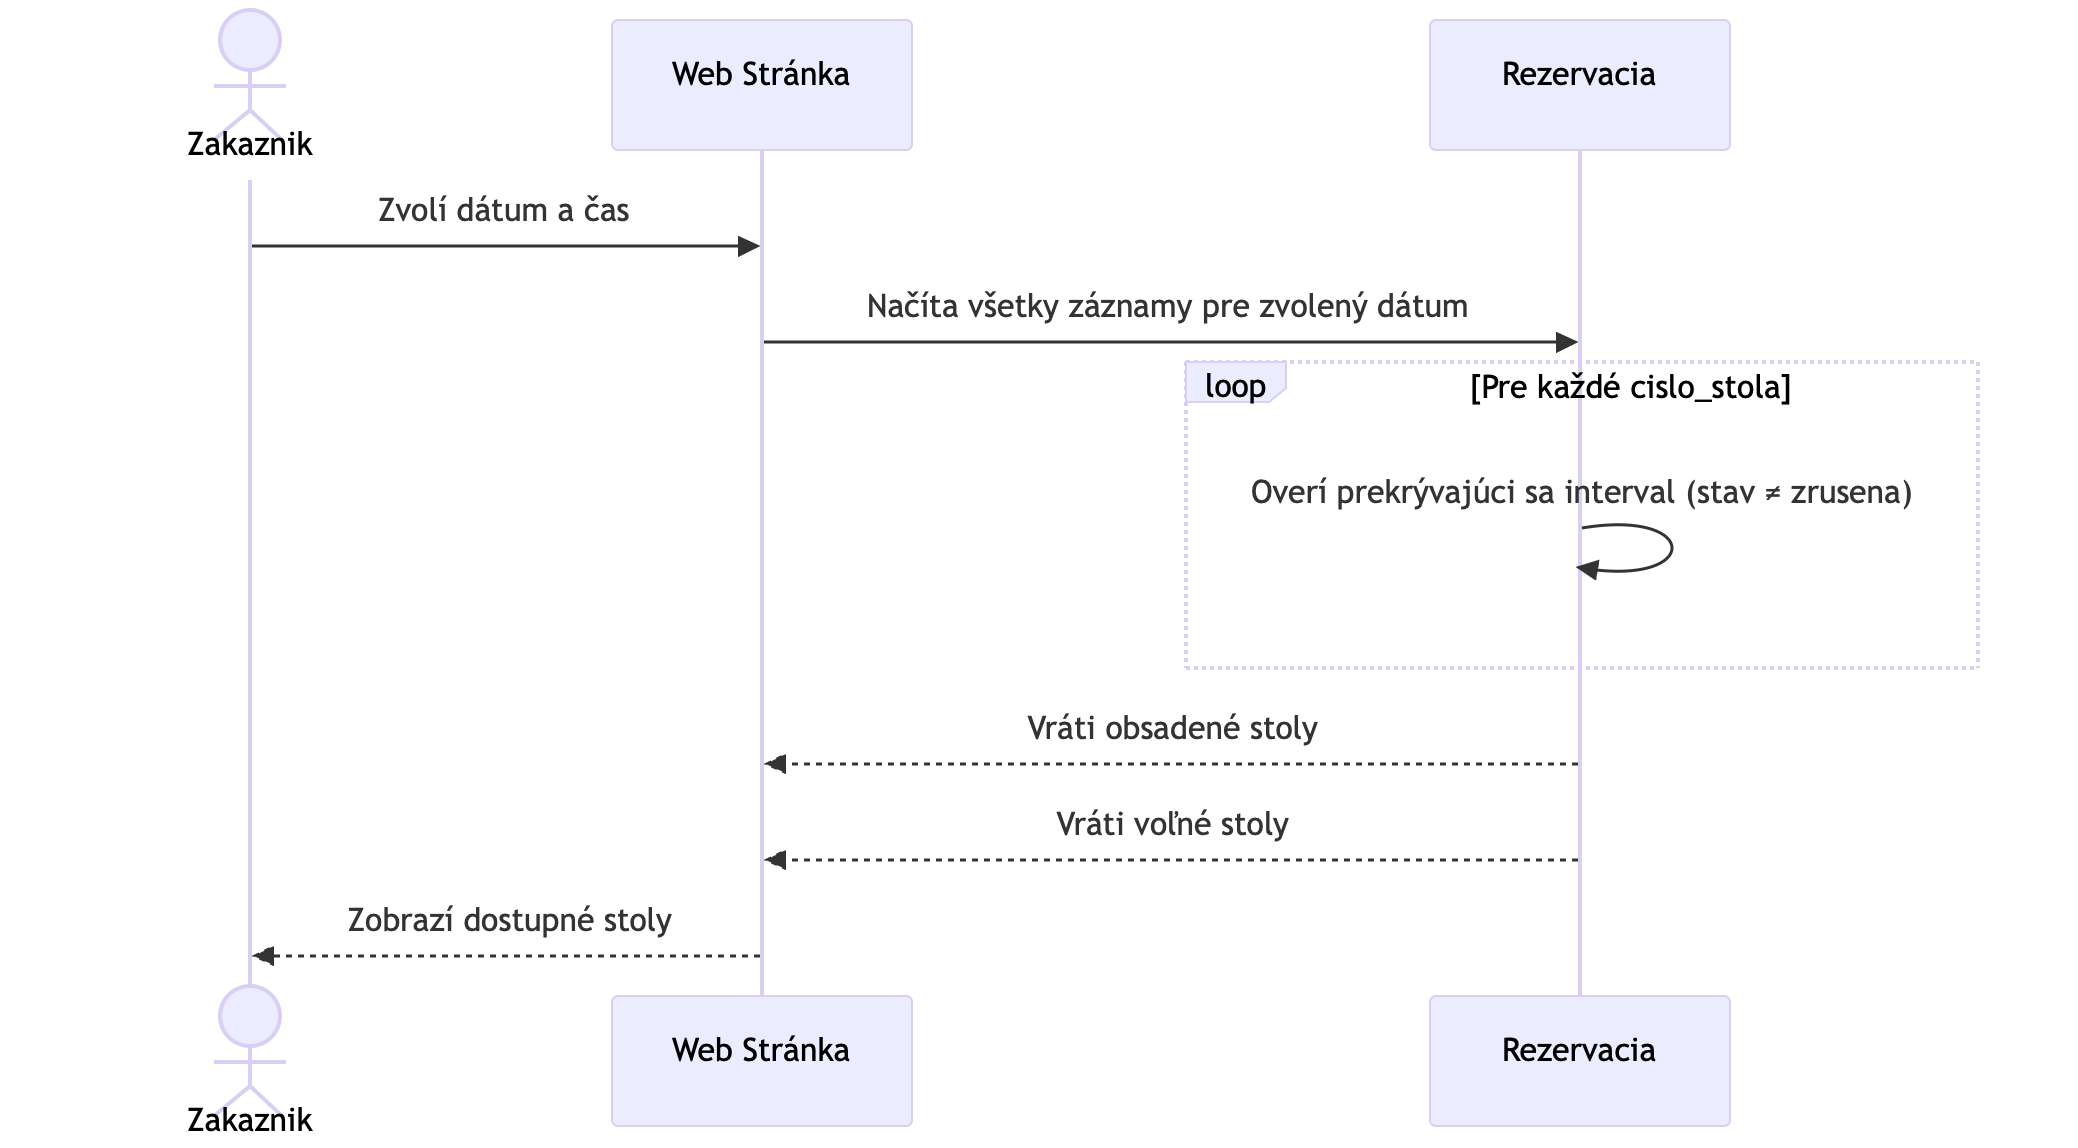
\includegraphics[width=\textwidth]{../assets/diagram1cast1}
    \caption{Scenár č.1 - Časť 1: Prezeranie dostupných stolov}
\end{figure}

\begin{figure}[H]
    \centering
    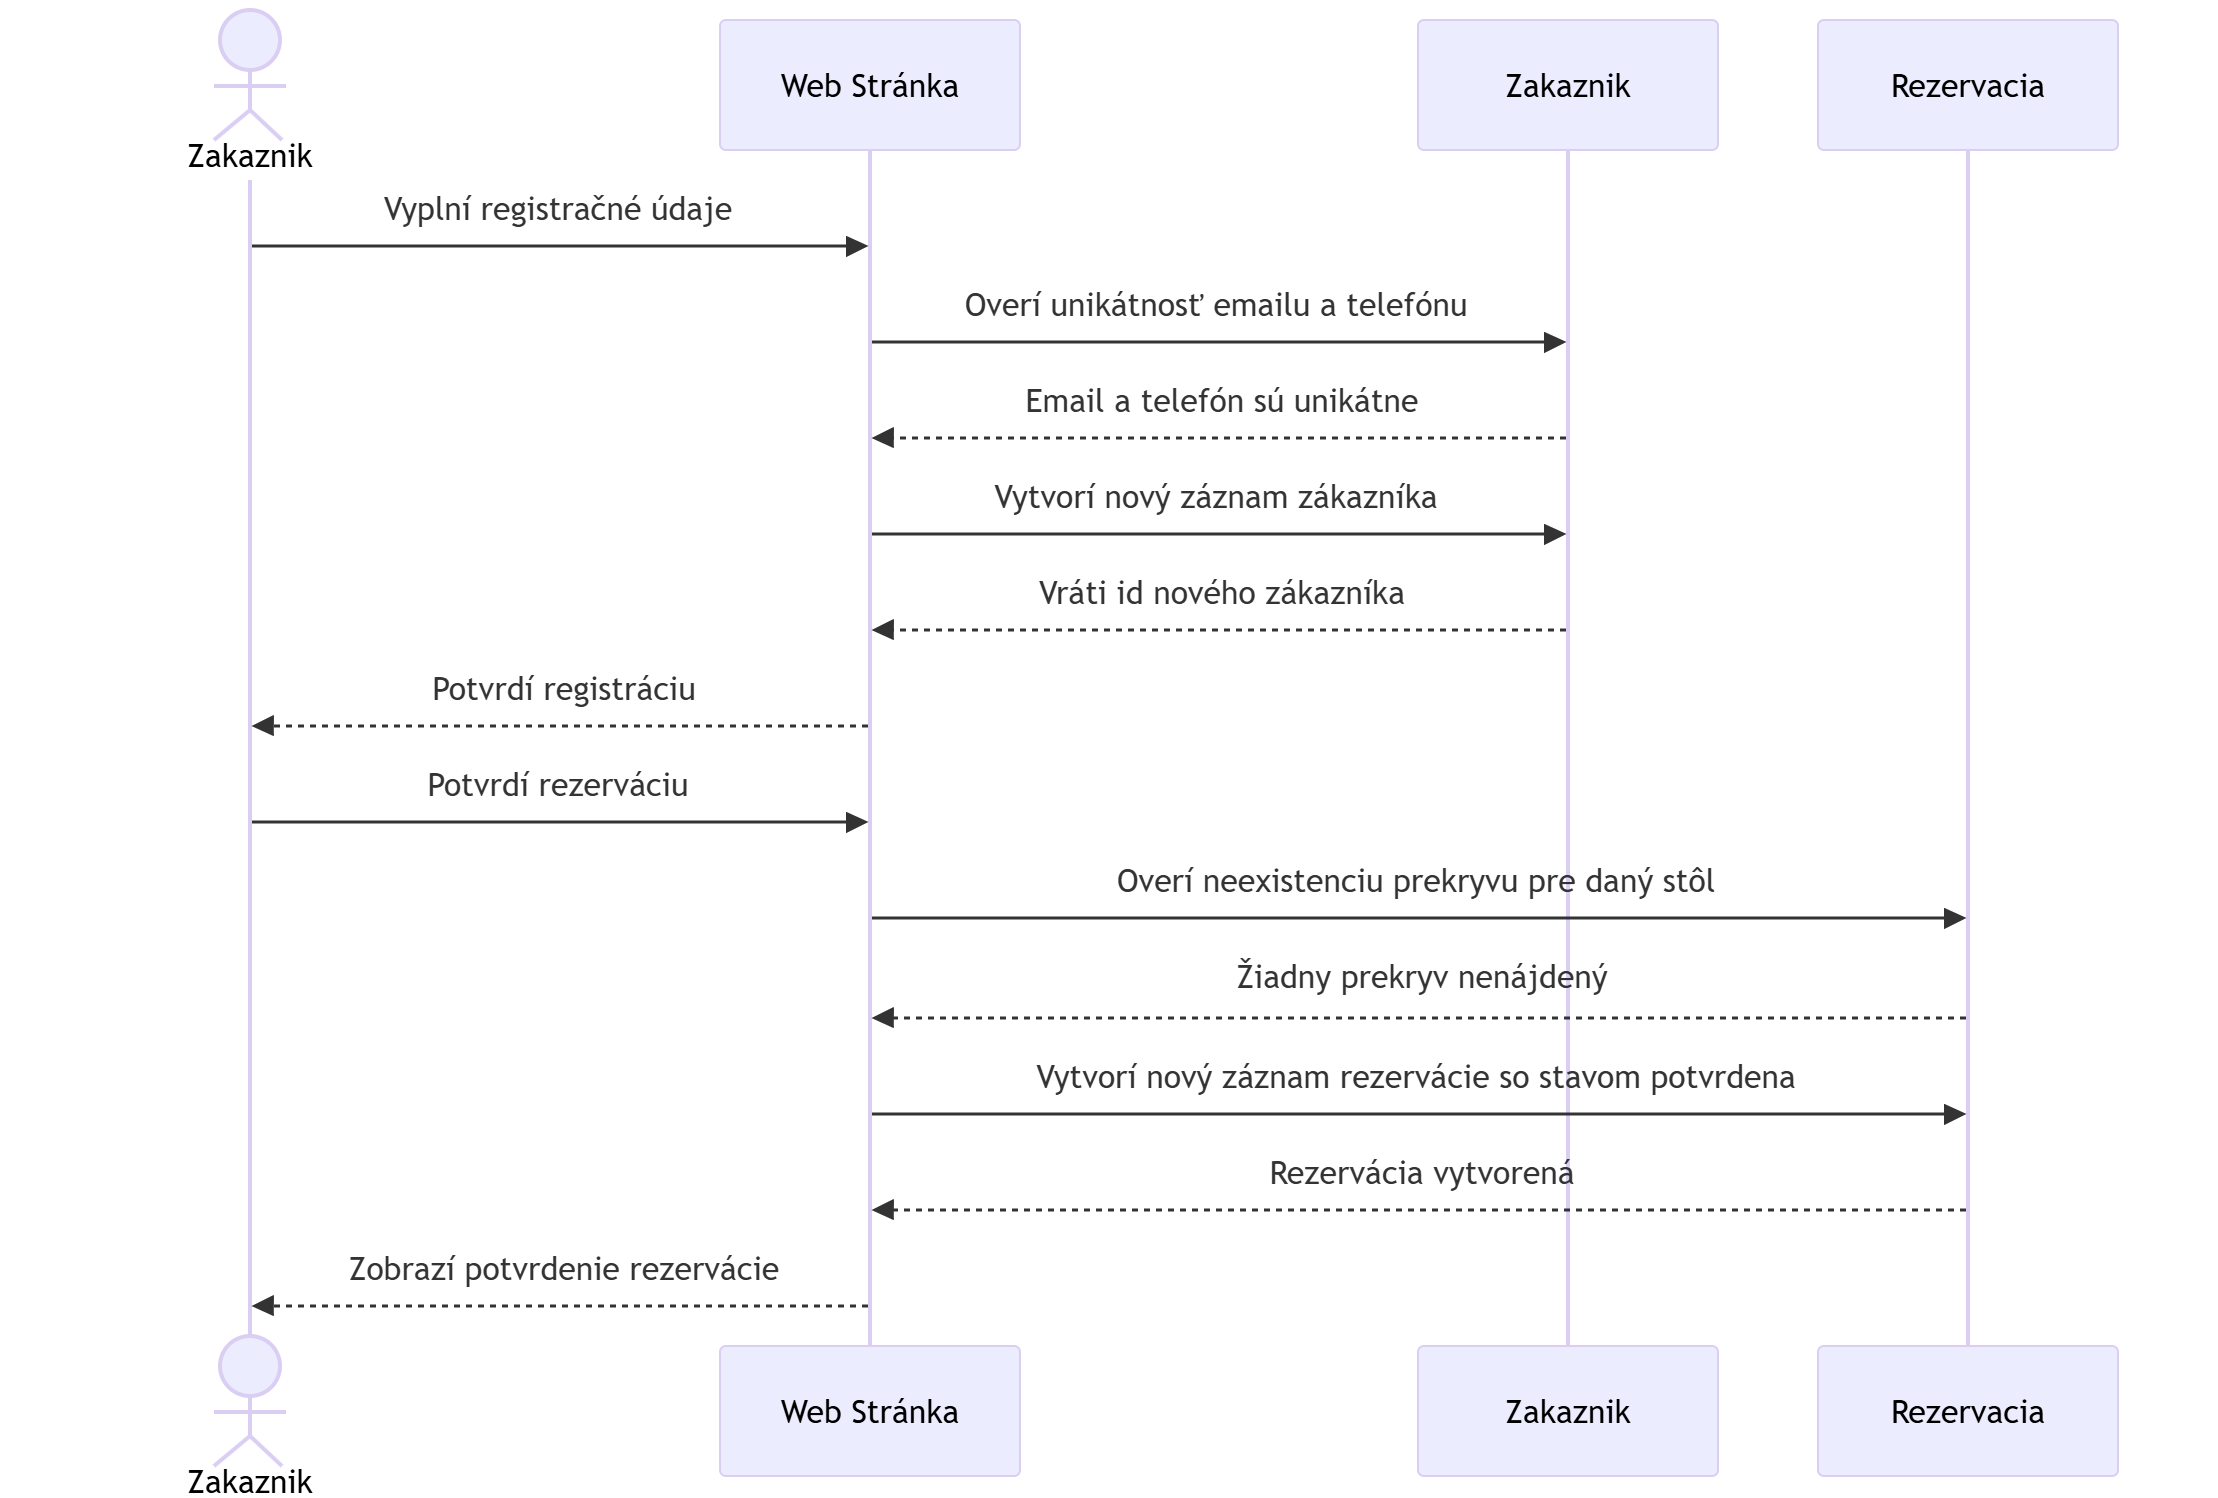
\includegraphics[width=\textwidth]{../assets/diagram1cast2}
    \caption{Scenár č.1 - Časť 2: Registrácia zákazníka a vytvorenie rezervácie}
\end{figure}

\begin{figure}[H]
    \centering
    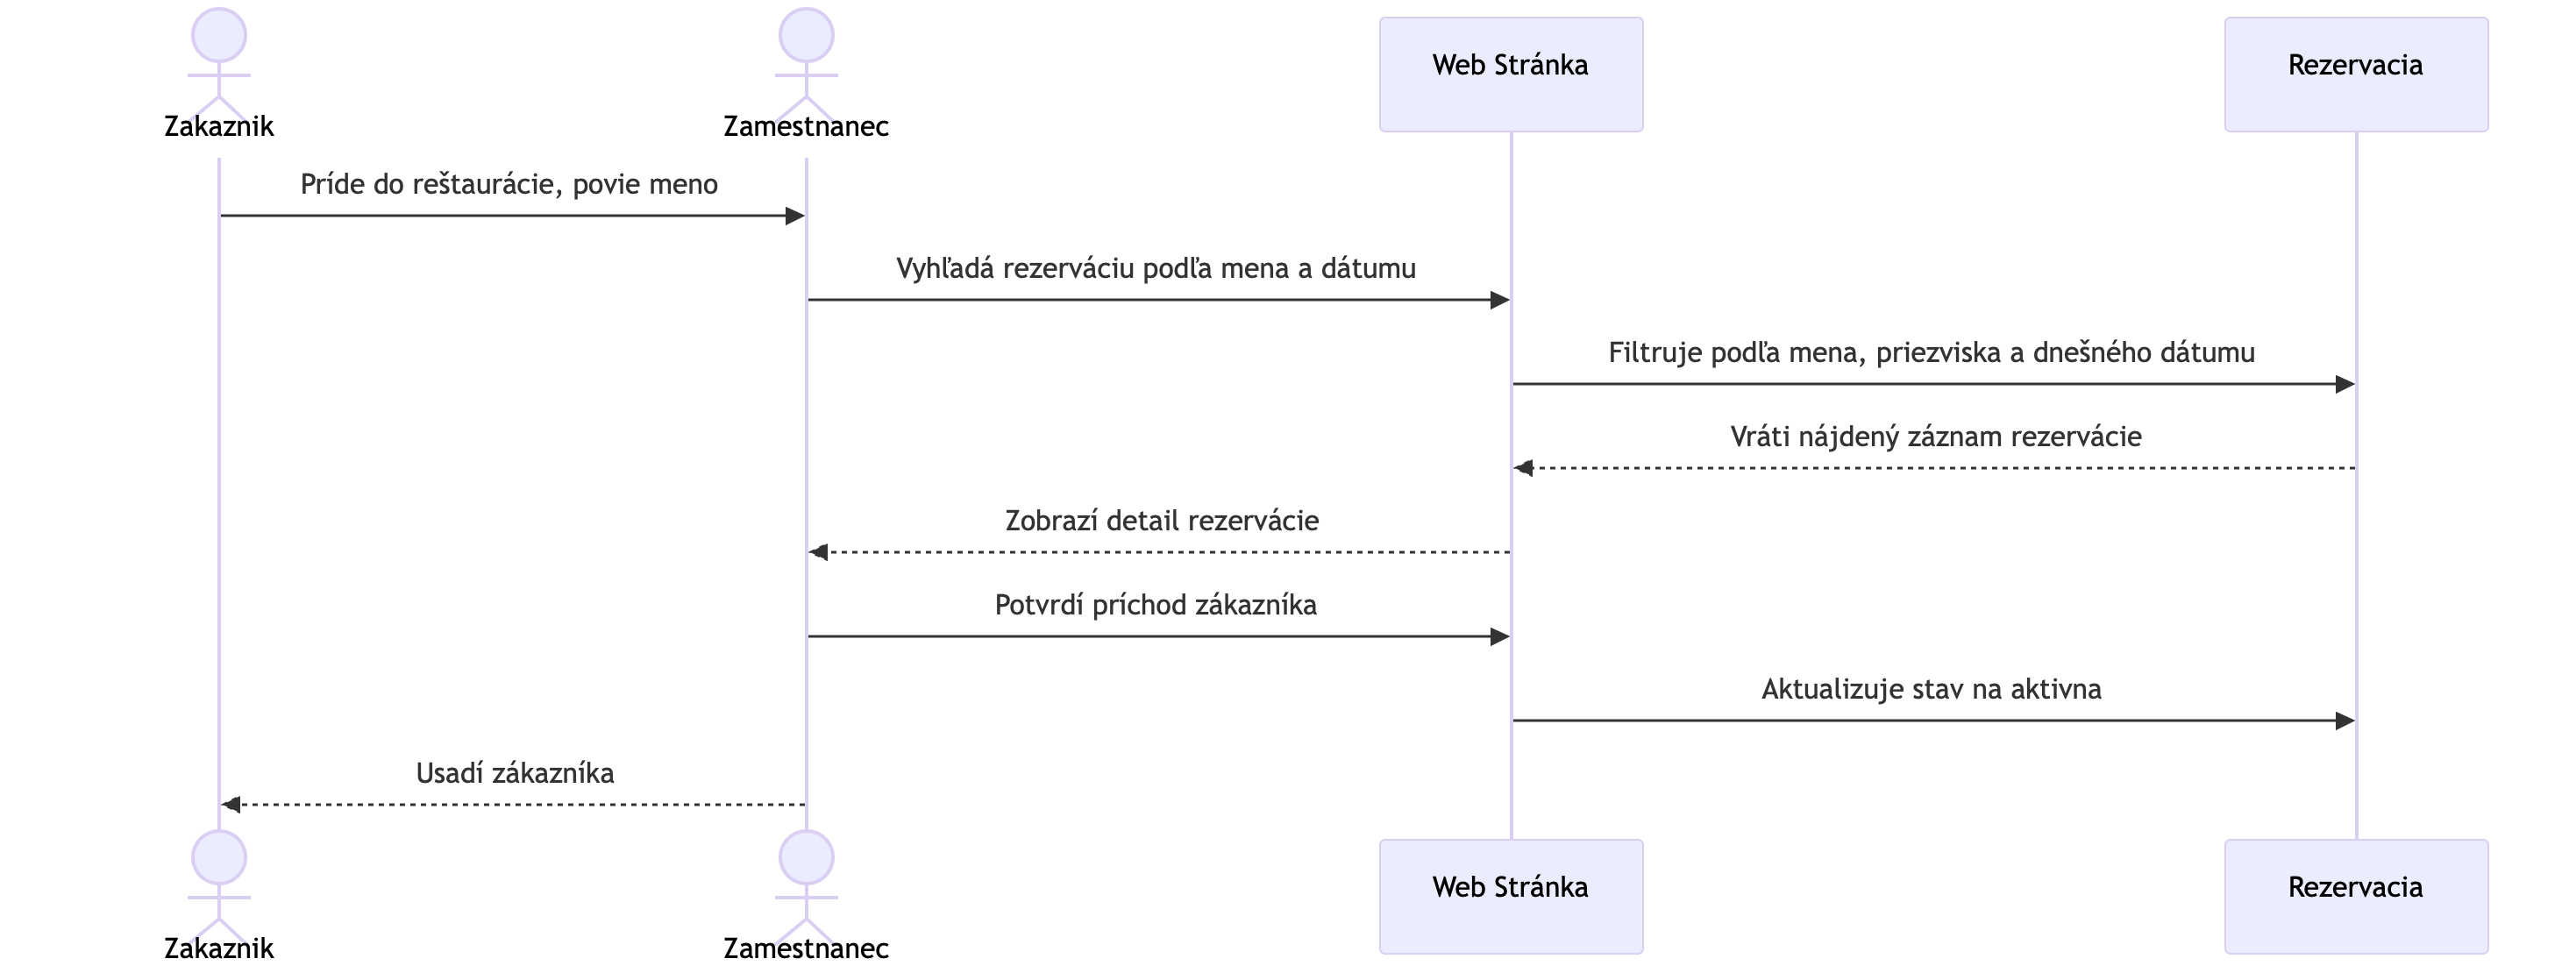
\includegraphics[width=\textwidth]{../assets/diagram1cast3}
    \caption{Scenár č.1 - Časť 3: Príchod do reštaurácie}
\end{figure}

% ─── Scenár 2 ─────────────────────────────────────

\begin{figure}[H]
    \centering
    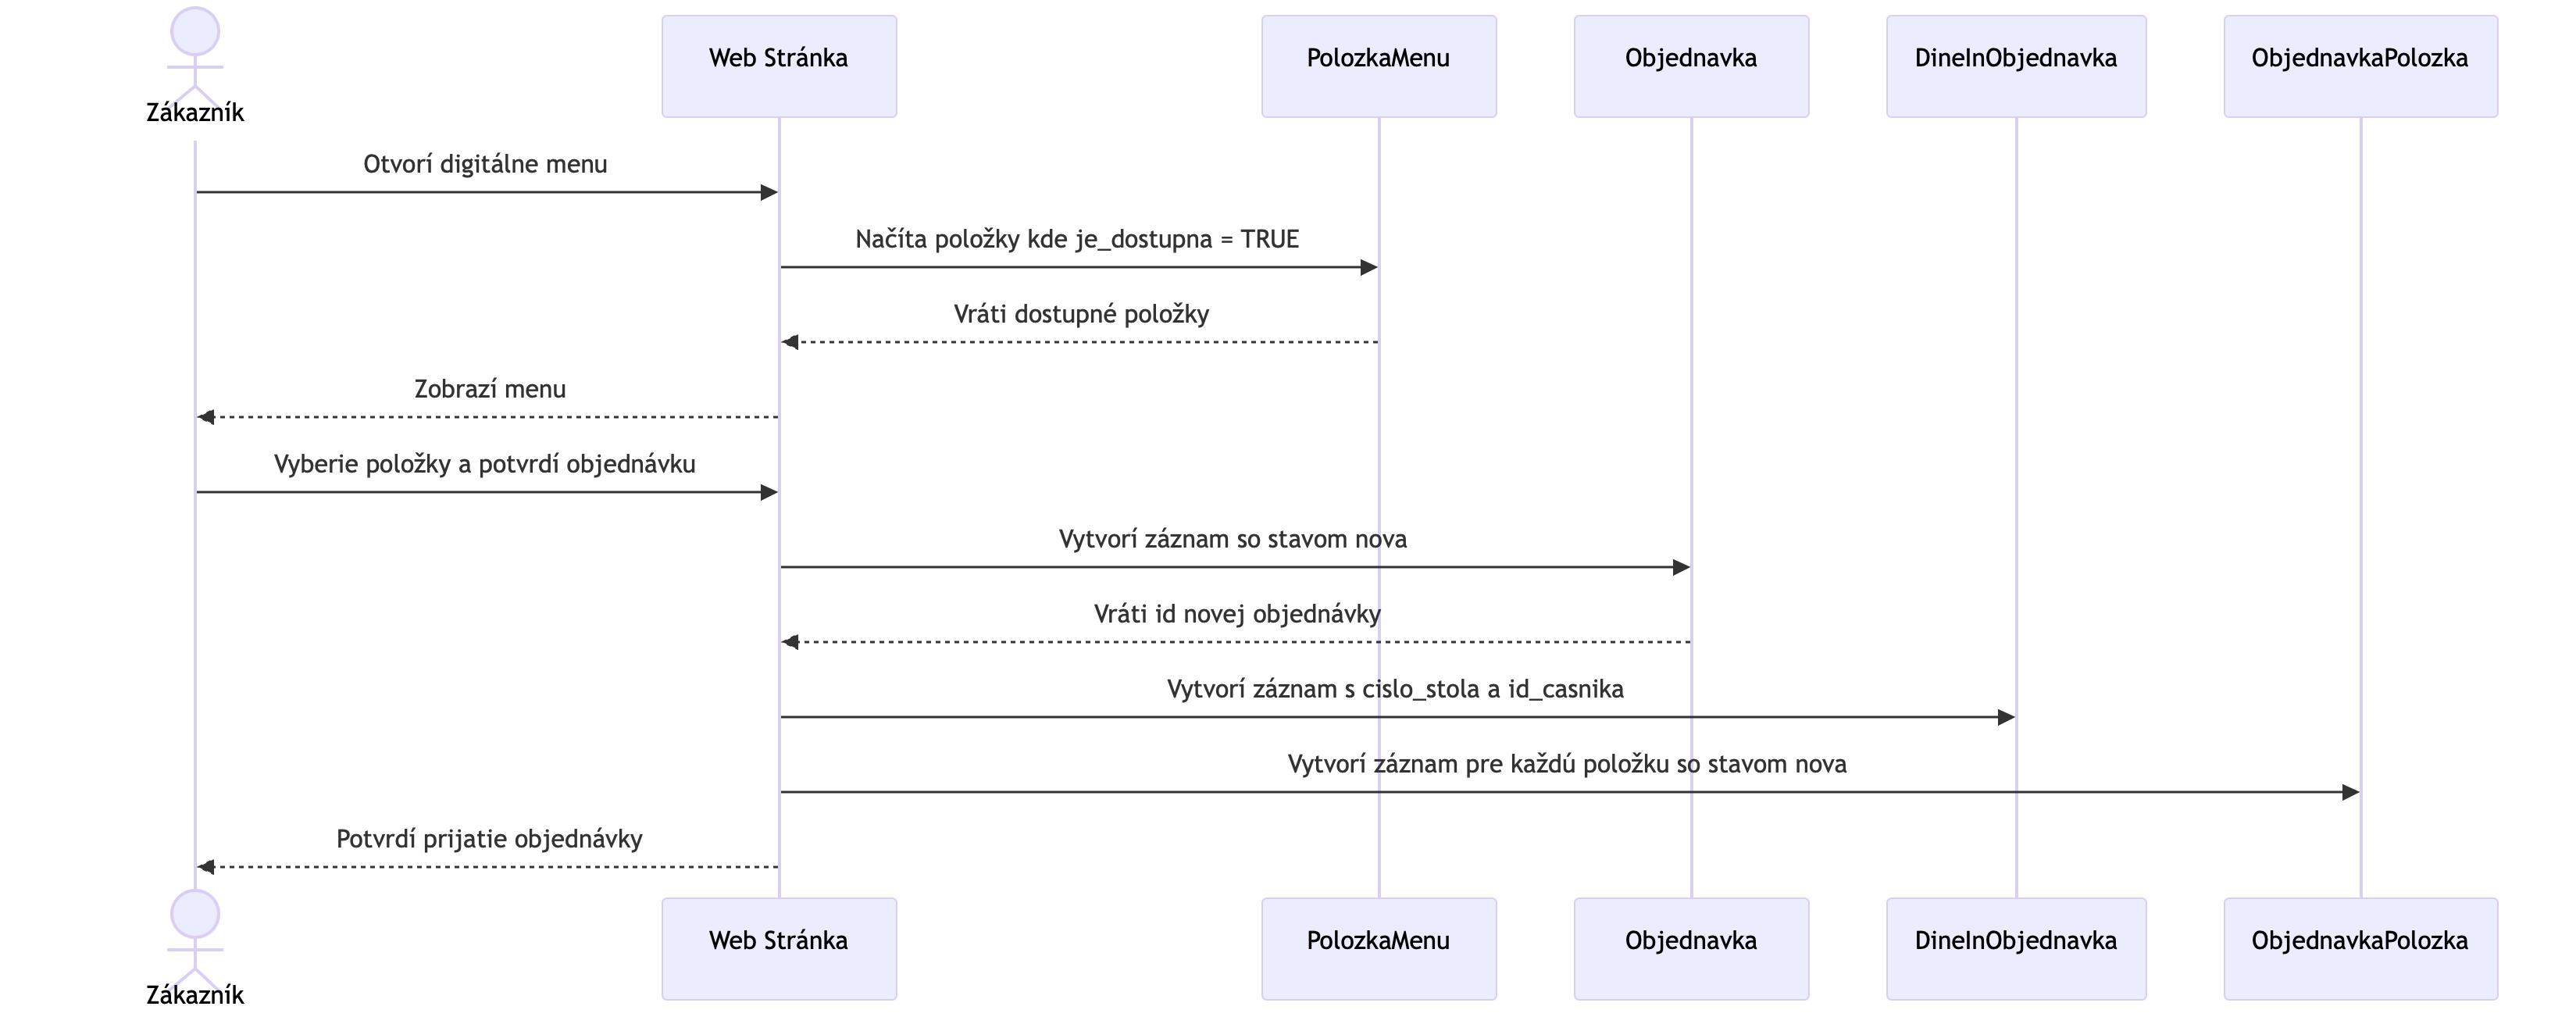
\includegraphics[width=\textwidth]{../assets/diagram2cast1}
    \caption{Scenár č.2 - Časť 1: Otvorenie menu a potvrdenie objednávky}
\end{figure}

\begin{figure}[H]
    \centering
    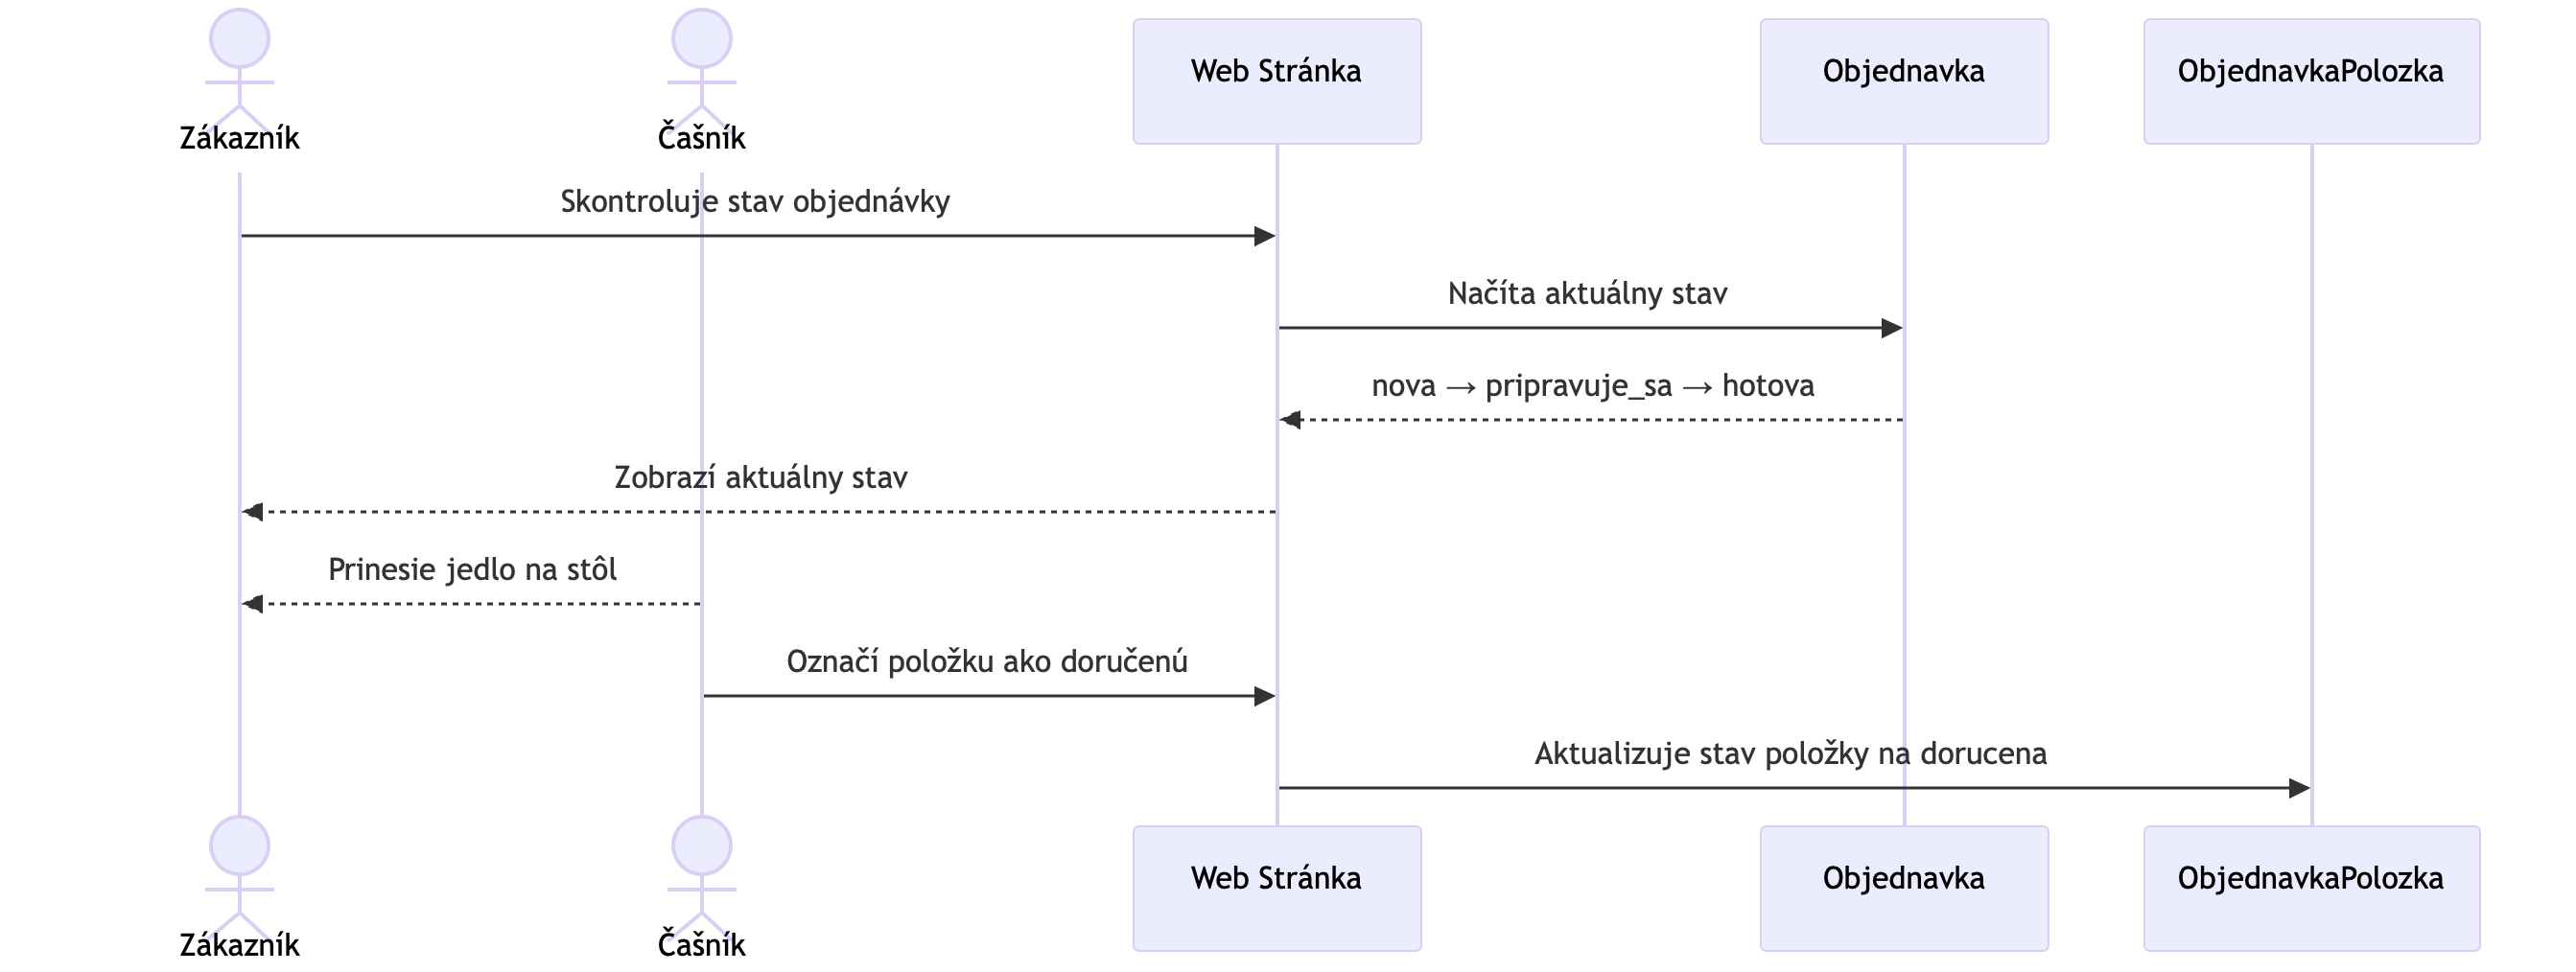
\includegraphics[width=\textwidth]{../assets/diagram2cast2}
    \caption{Scenár č.2 - Časť 2: Sledovanie stavu a doručenie jedla}
\end{figure}

\begin{figure}[H]
    \centering
    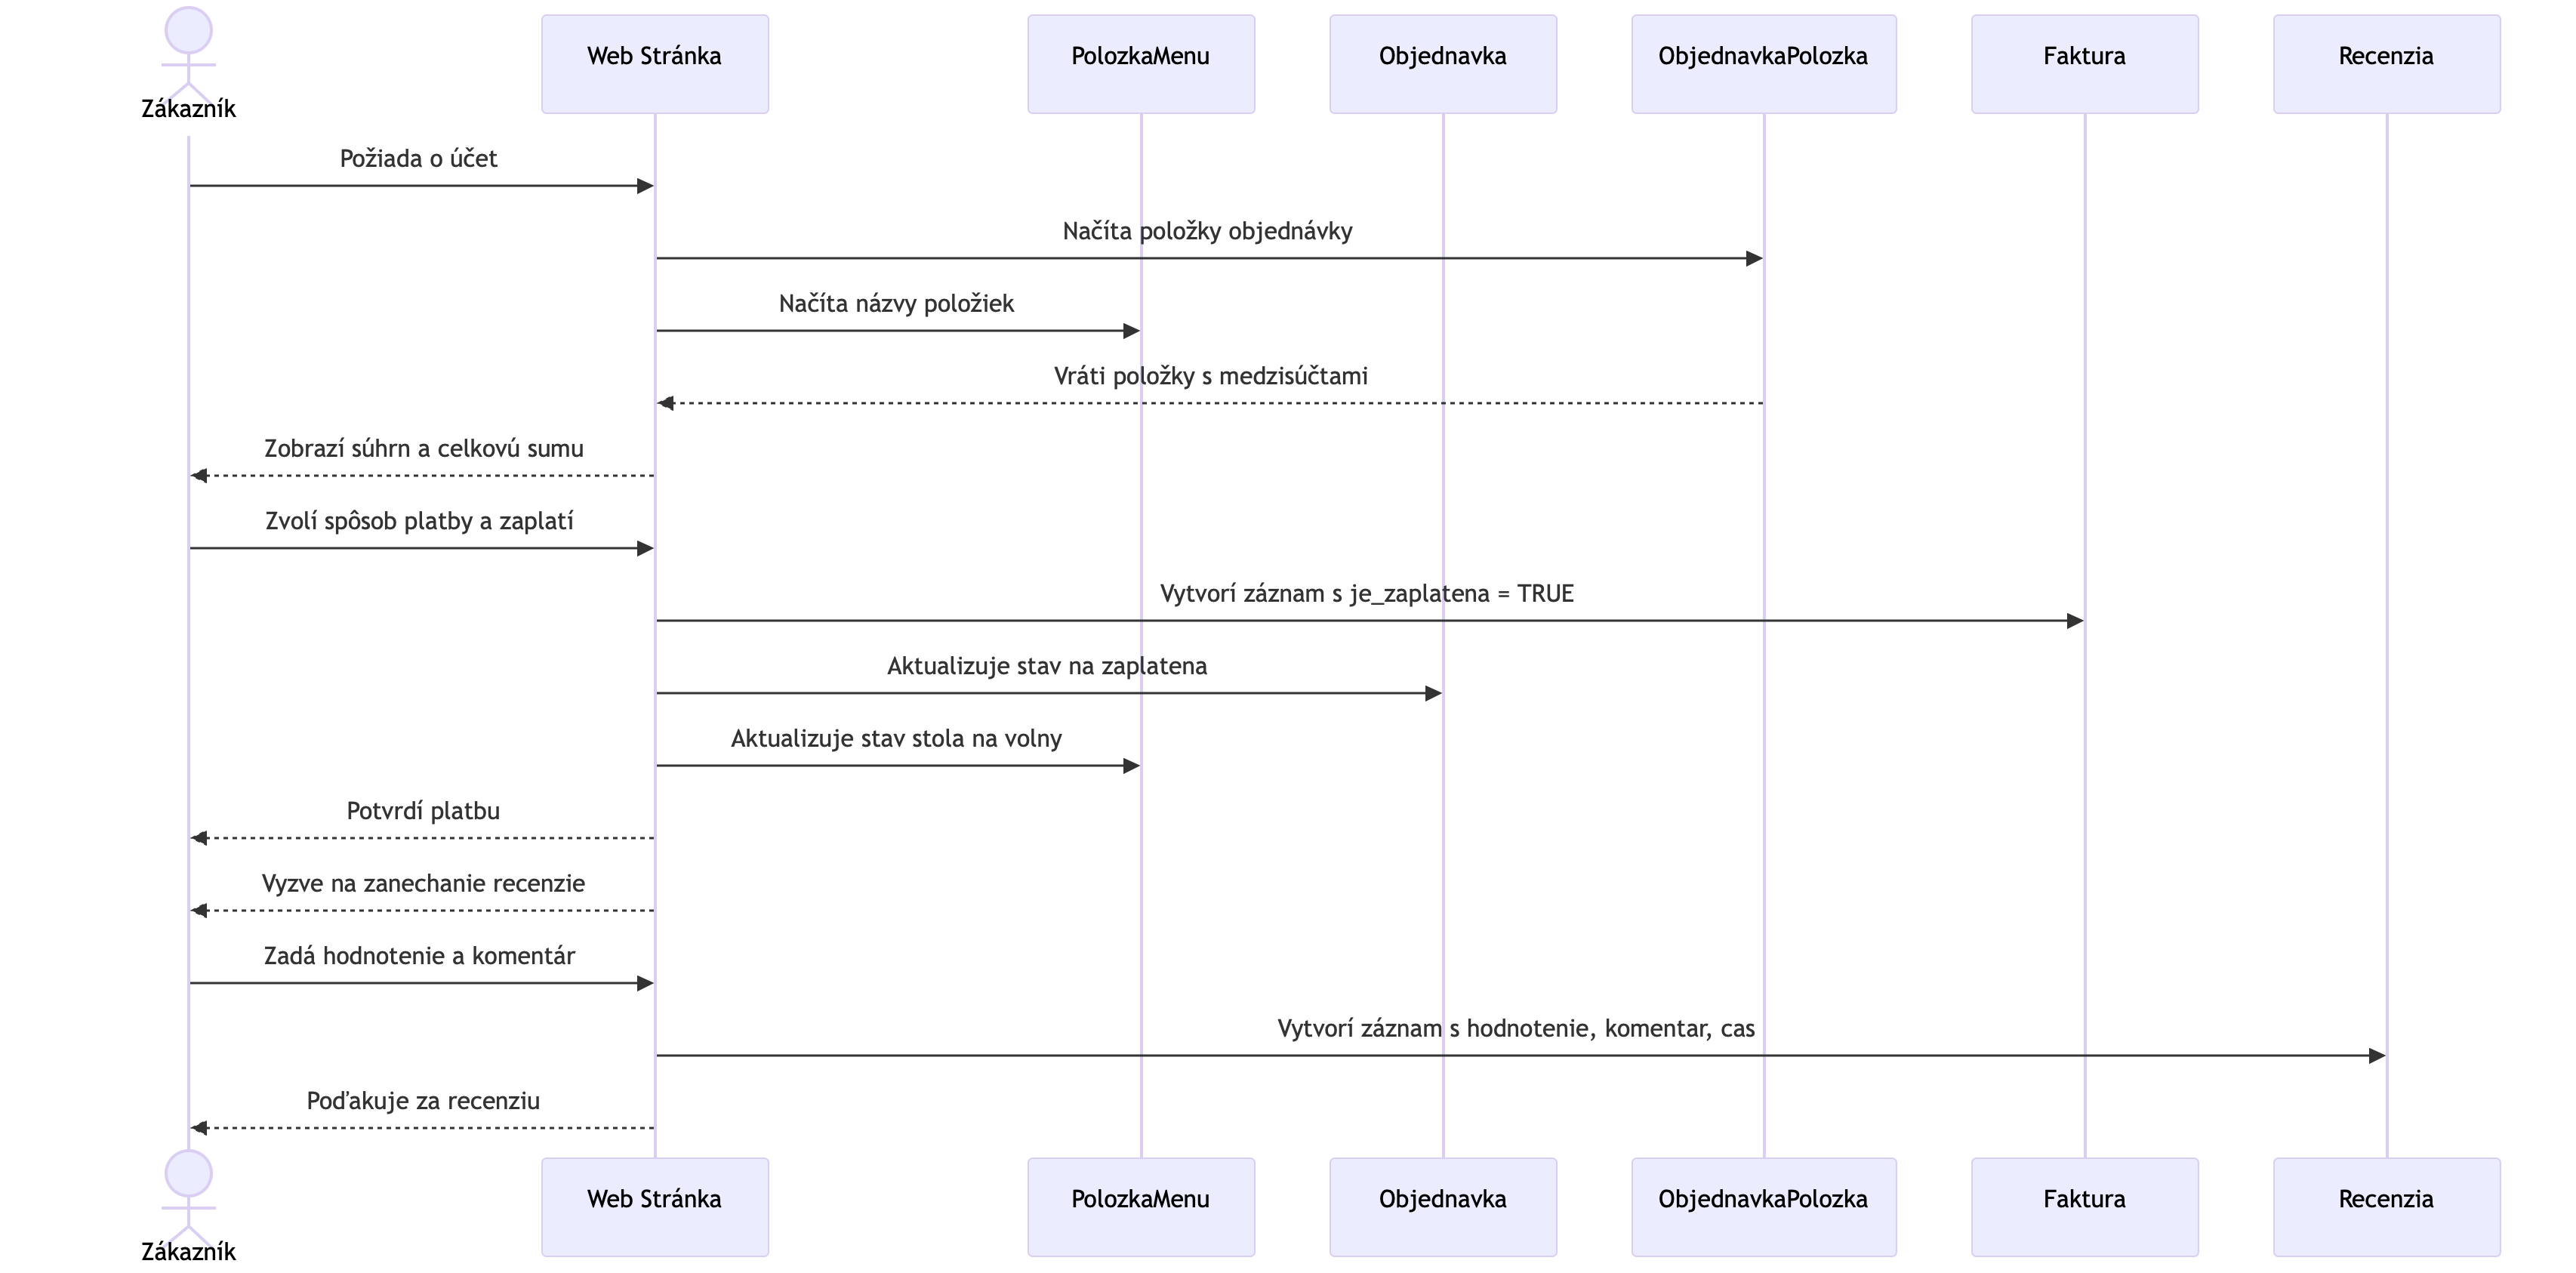
\includegraphics[width=\textwidth]{../assets/diagram2cast3}
    \caption{Scenár č.2 - Časť 3: Účet, platba a recenzia}
\end{figure}

% ─── Scenár 3 ─────────────────────────────────────

\begin{figure}[H]
    \centering
    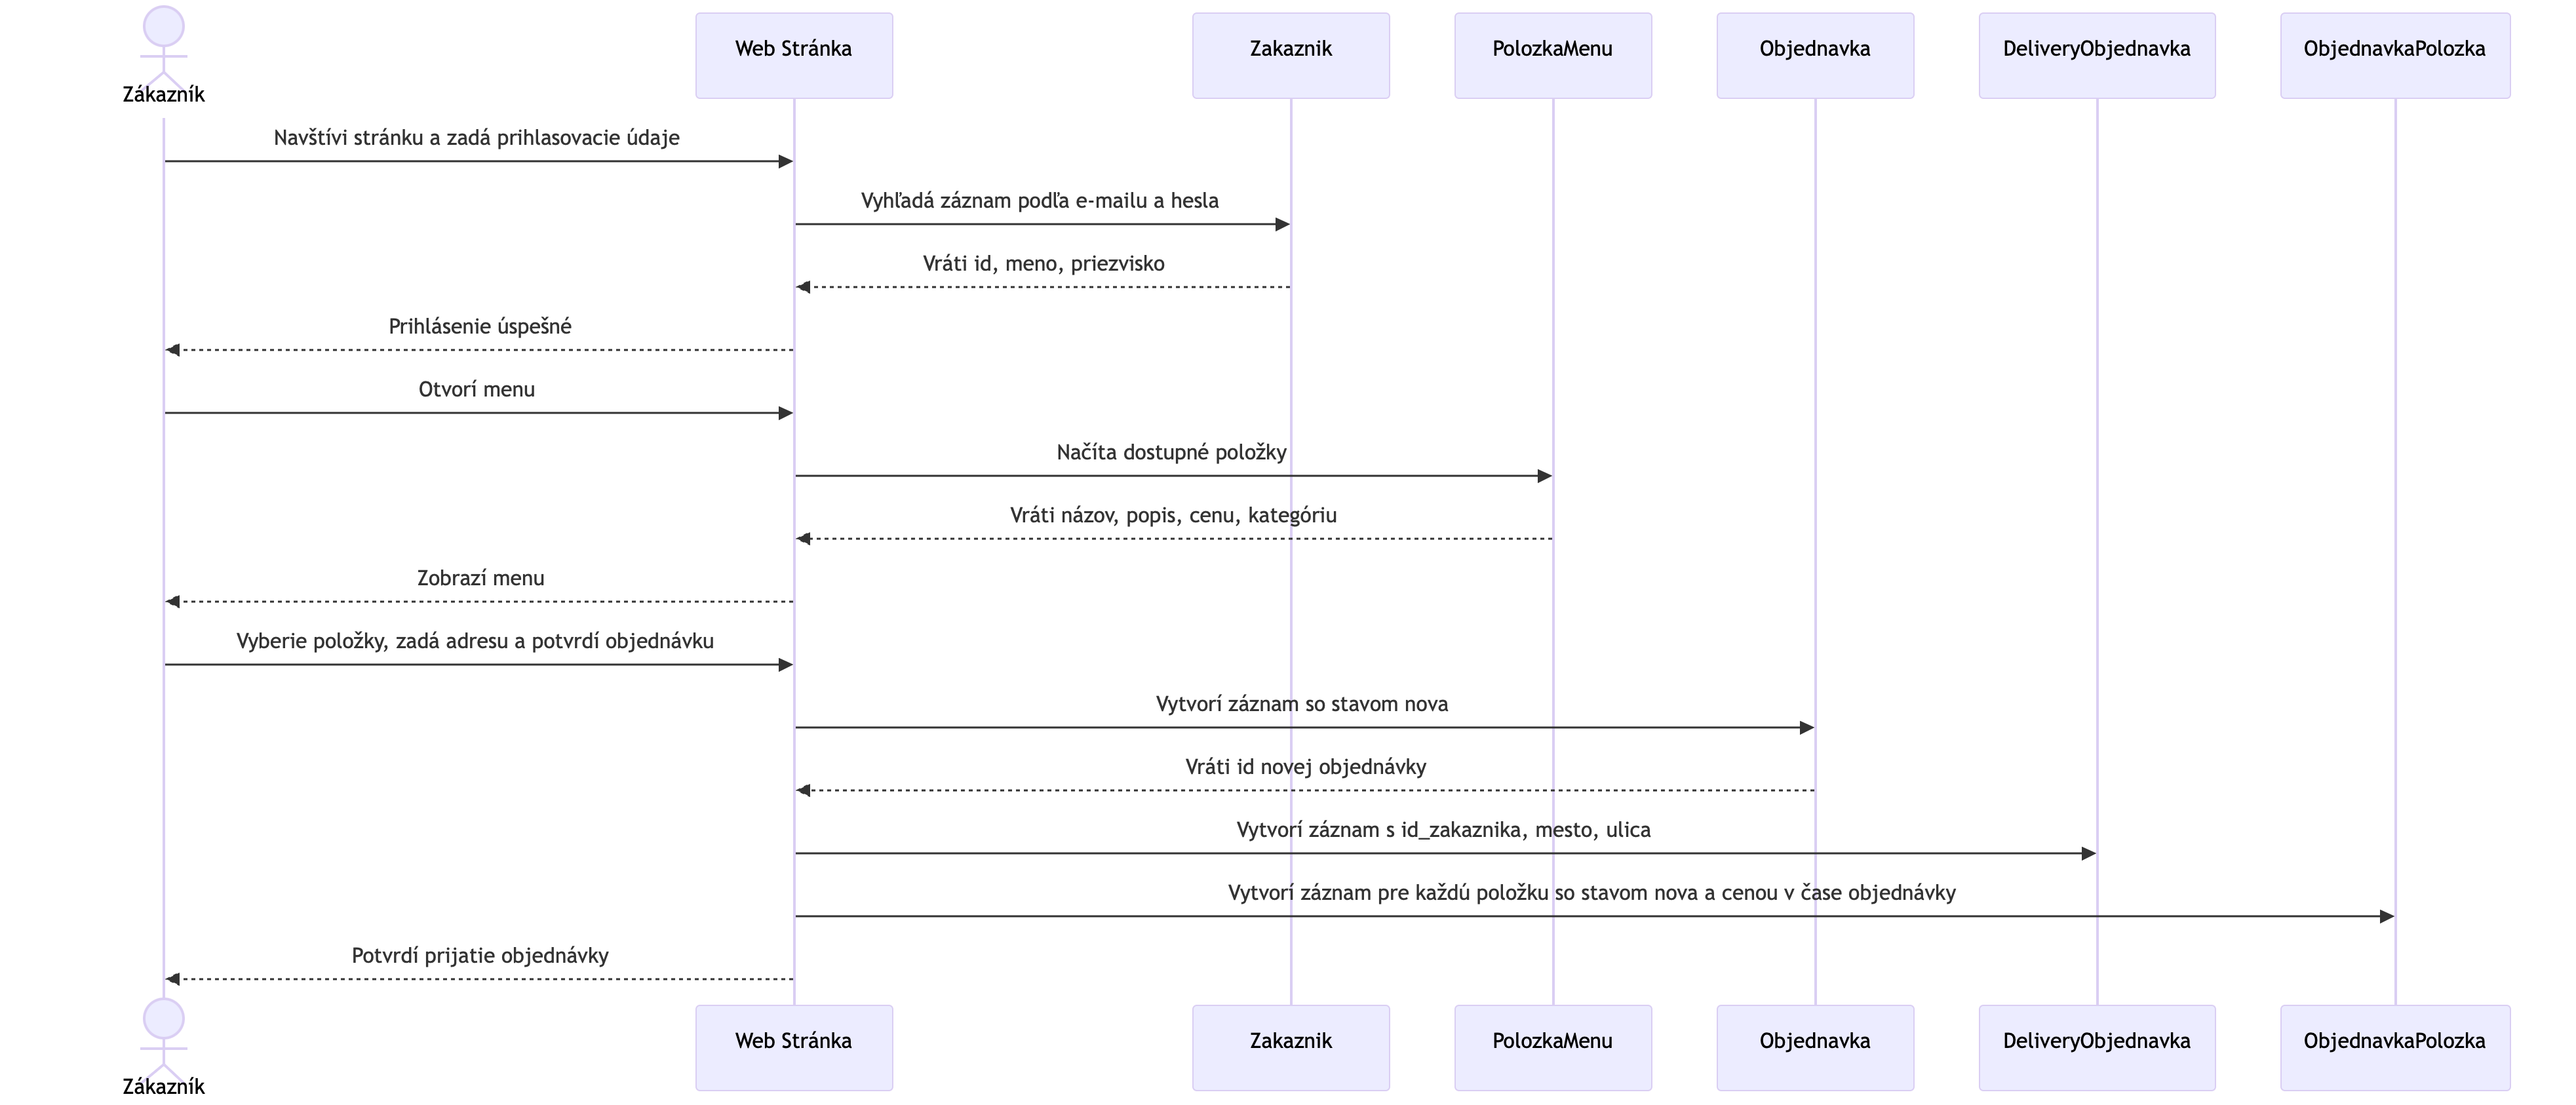
\includegraphics[width=\textwidth]{../assets/diagram3cast1}
    \caption{Scenár č.3 - Časť 1: Prihlásenie, výber položiek a potvrdenie objednávky}
\end{figure}

\begin{figure}[H]
    \centering
    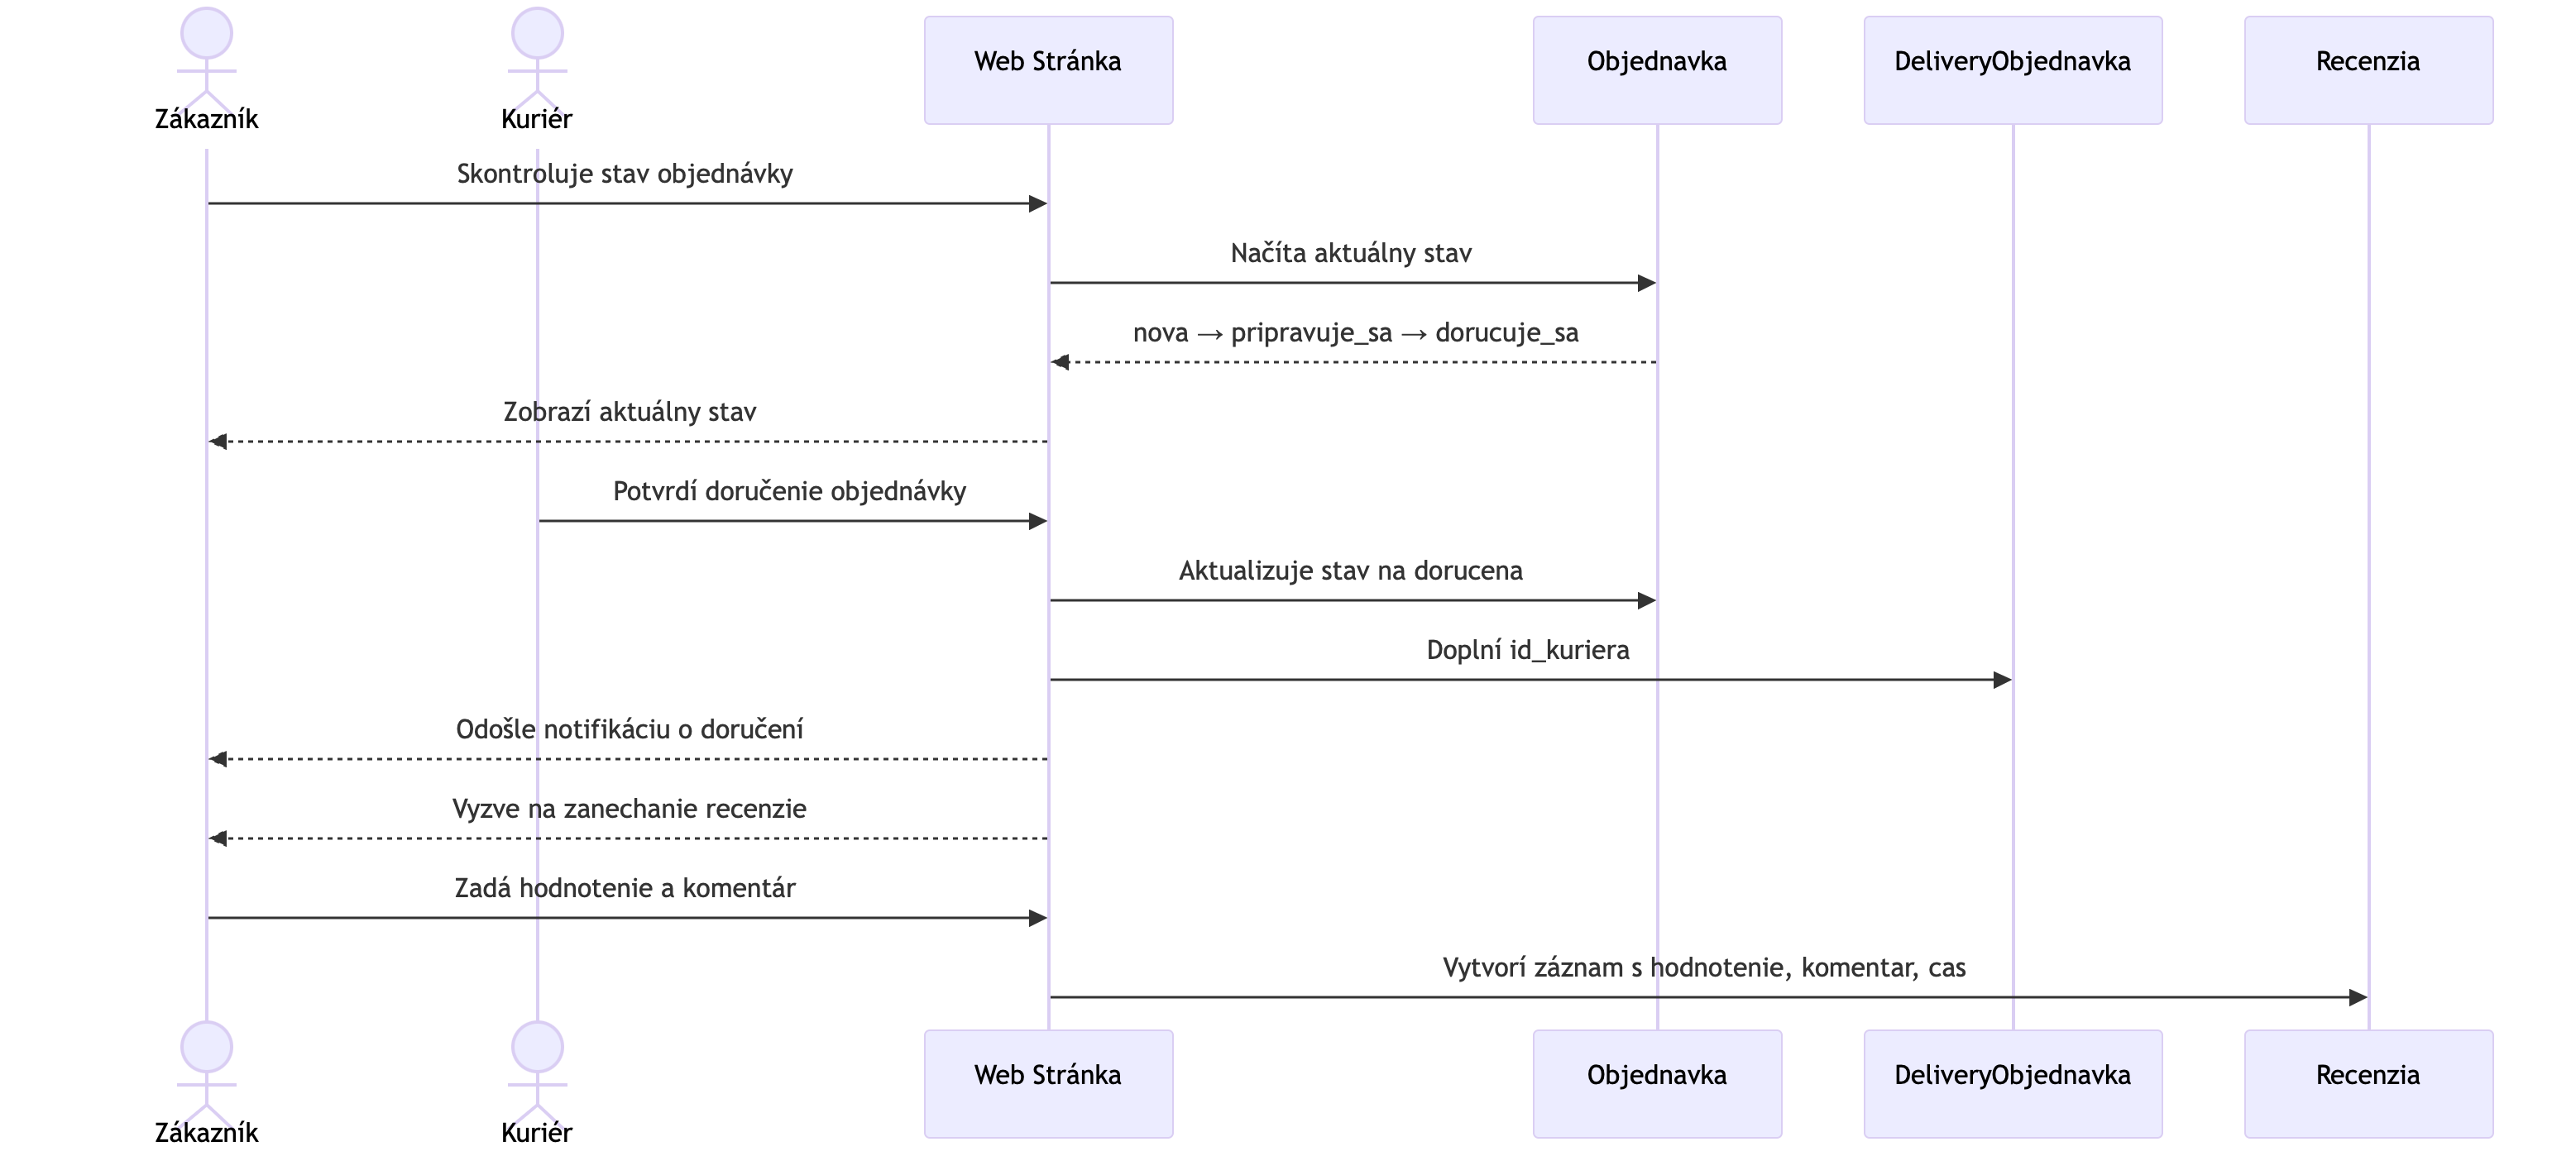
\includegraphics[width=\textwidth]{../assets/diagram3cast2}
    \caption{Scenár č.3 - Časť 2: Sledovanie stavu, doručenie a recenzia}
\end{figure}

% ─── Scenár 4 ─────────────────────────────────────

\begin{figure}[H]
    \centering
    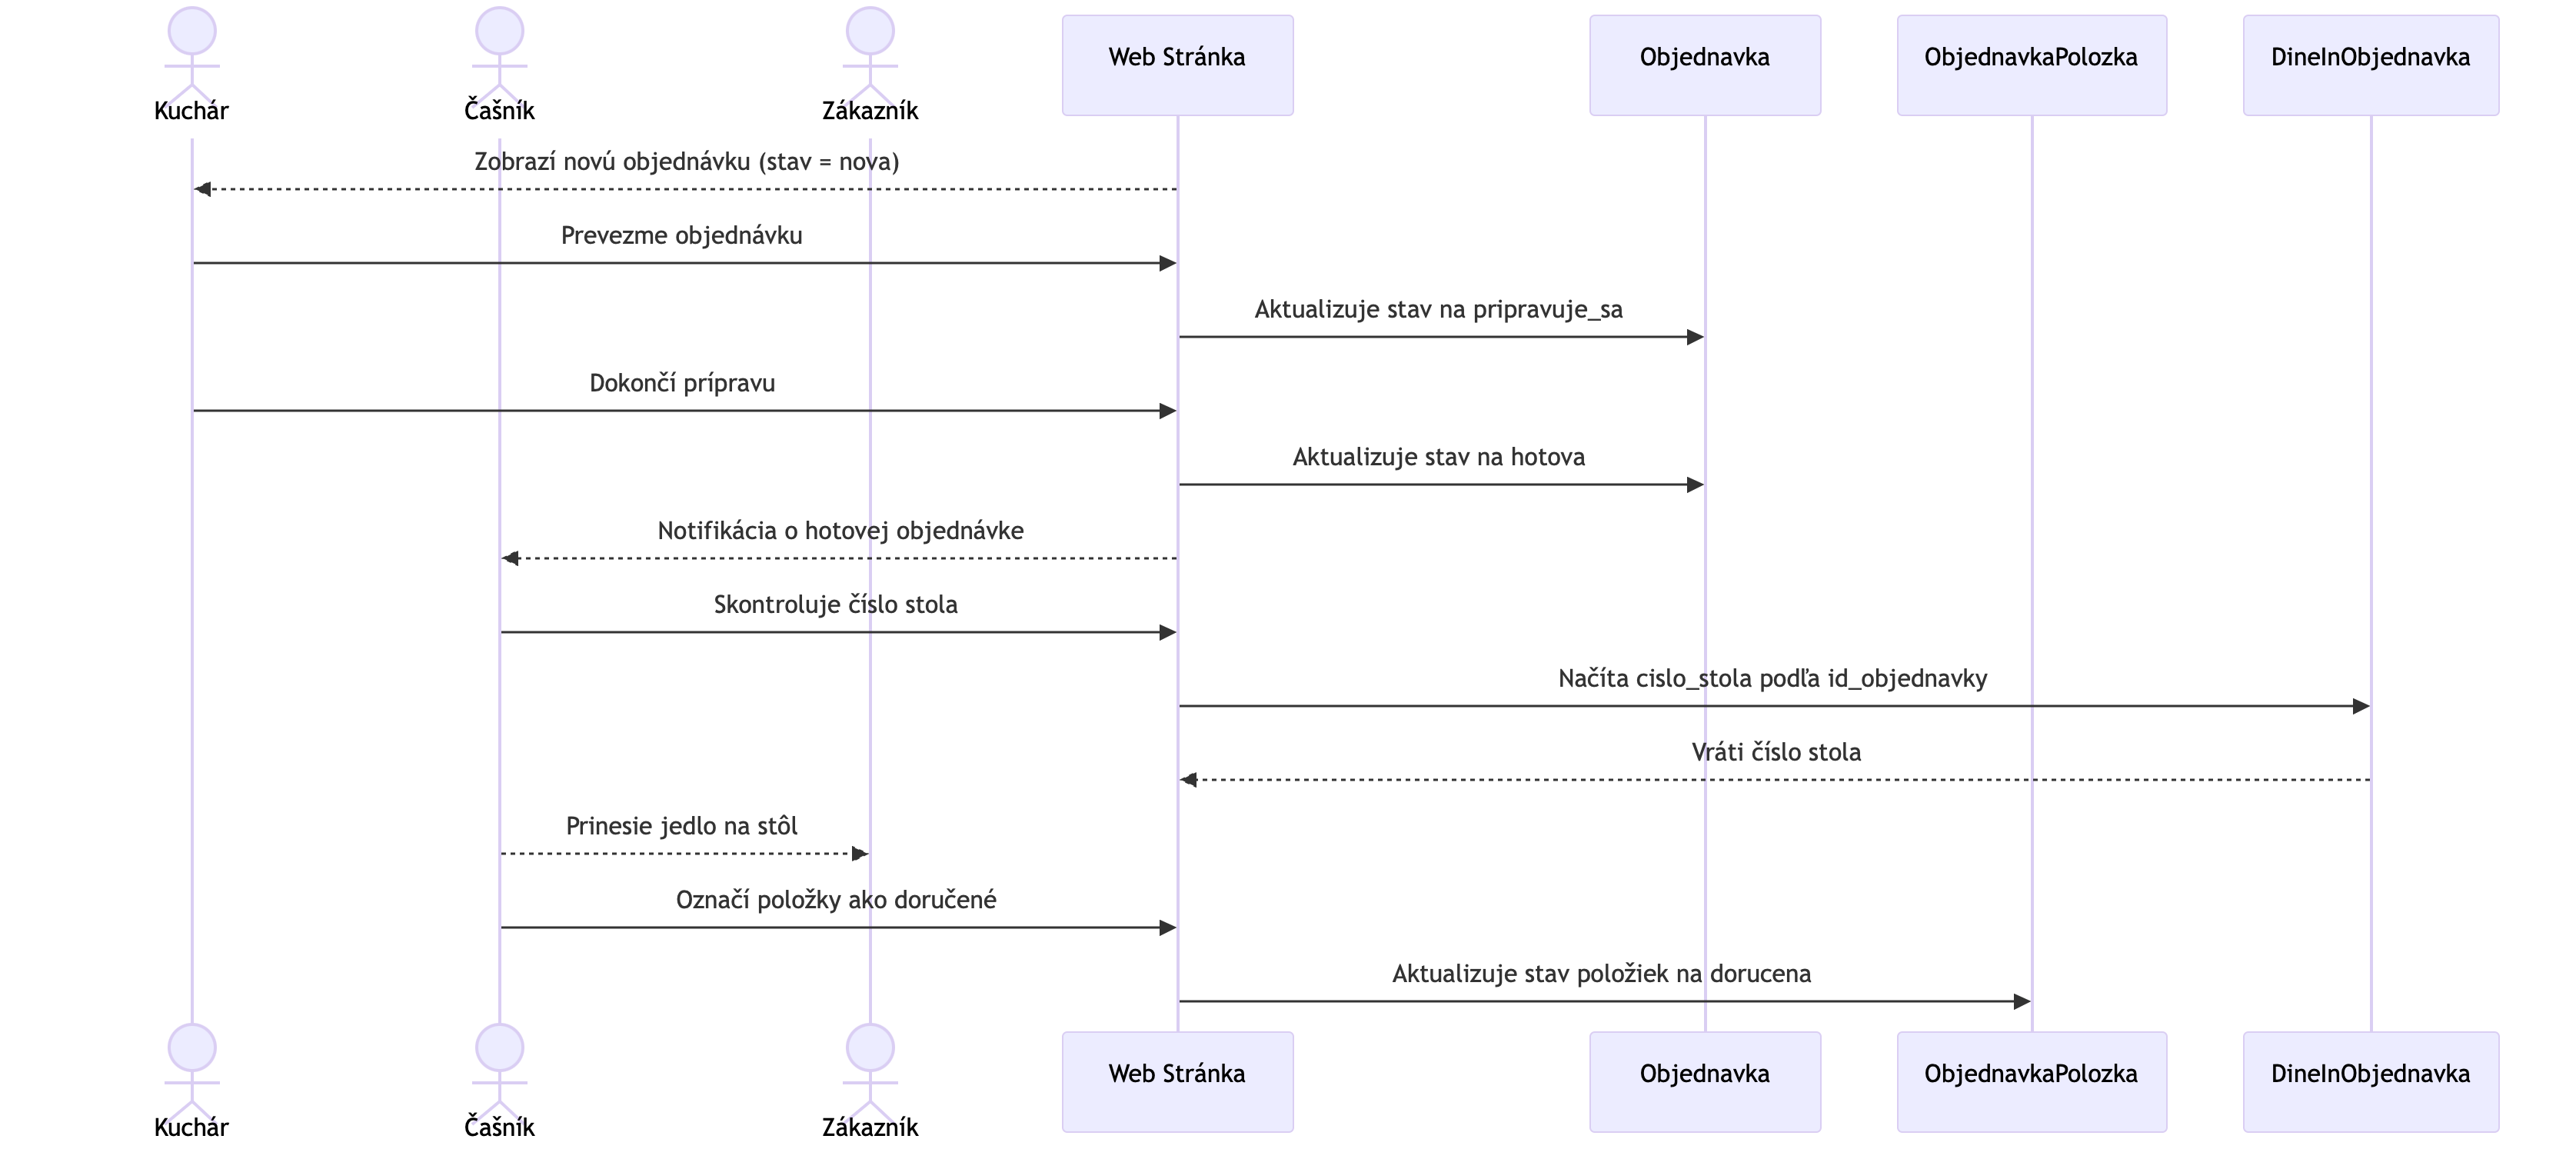
\includegraphics[width=\textwidth]{../assets/diagram4cast1}
    \caption{Scenár č.4 - Príprava objednávky kuchárom a výdaj čašníkom}
\end{figure}

\end{document}